%%%%%%%%%%%%%%%%%%%%%%%%%%%%%%%%%%%%%
\chapter{CMS Resistive Plate Chambers - RPC}
\label{chapter_rpc}

In the course of this PhD study, there were a lot of opportunities to work for the RPC project, in the context of the CMS Collaboration. The main activities consists of shifts for the RPC operation and data certification, upgrade and maintenance of the online software, R\&D activities for the RPC upgrade and detector maintenance during the LHC Long Shutdown 2 (2019 to 2020).

In this chapter, it is presented a summary of the Resistive Plate Chamber technology and the contributions to the RPC project at CMS.

\section{Resistive Plate Chambers}

The seminal paper on the Resistive Plate Chamber (RPC) technology was presented by R. Santonico and R. Cardarelli, in which they described a "dc operated particle detector (...) whose constituent elements are two parallel electrode Bakelite plates between"~\cite{rpc_seminal}. The key idea behind the RPC, with respect to other similar gaseous detectors, is the use of two resistive plates as anode an cathode, which makes possible to have a small localized region of dead time, achieving very good time resolution. 

The working principle for RPCs relies on the idea that a ionizing particle crossing the detector, tend to interact with the gap between the two plates (filled with some specific gas mixture) and form a ionizing cascade process, in which the produced charged particle are driven by the strong uniform electrical field produced by the two plates.

The gas mixture is a key component of a RPC. Even though the first RPCs were produced with a mixture of argon and butane, nowadays RPCs use a mixture of gases that would enhance an ionization caused by the incident particle and quench secondary (background) effects.

Another feature of the RPCs is its construction simplicity and low cost. This allow the use RPC to cover larger at a reasonable cost. 

A extensive review of the RPC technology and its application can be found at~\cite{livro_rpc}.

\subsection{Principles and operation modes}

The core of a RPC chamber is a gap made with two parallel high resistivity plates, separated by some regular distance (typically millimeters), filled with with a proper gas mixture and under appropriate high voltage (HV) applied on the plates (electrodes, from here on). When a ionizing particle crosses the gap, there is a high enough chance the the particle will interact with the gas and produce a newly created positive ion and a electron. This pair will travel in opposite directions, according to the electric field from the electrodes. During this process, the electron will gain kinetic energy and inelasticly interact with other neighboring atoms/molecules, creating excitations in their energy levels and, potentially, also ionizing them. The secondary ionization electrons will also follow the same curse, creating an \textbf{Avalanche} of positive and negative particle/ions traveling towards the electrodes. This process is proportional to the applied electric field. Figure~\ref{avalanche} illustrates the avalanche production.


\begin{figure}[h]
    \begin{center}
    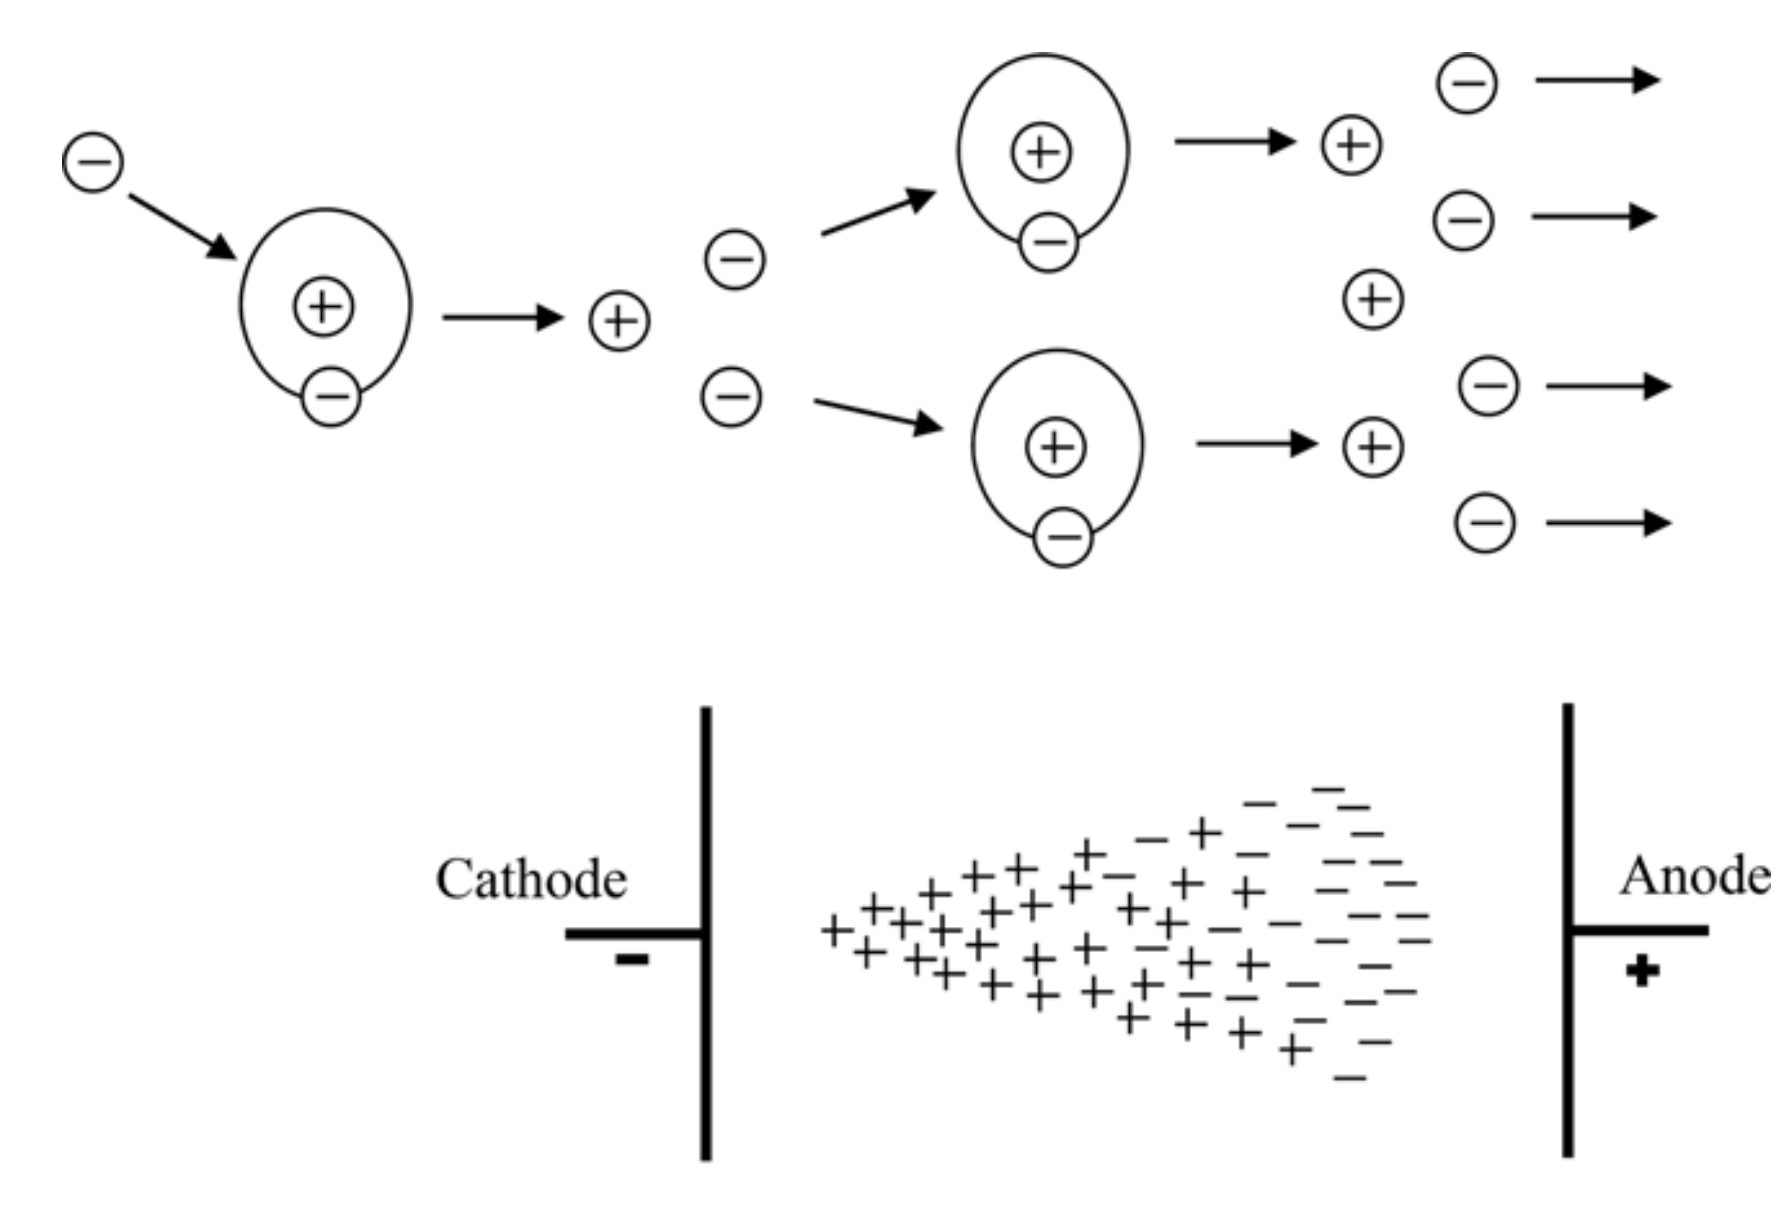
\includegraphics[width=0.5\textwidth,keepaspectratio]{figures_and_tables/rpc/avalanche_prod.png}
    \end{center}
    \caption{The Avalanche production process inside a RPC gap. (Top) The initial process and the secondary electron/ion generation. (Bottom) The overall charge distribution of an Avalanche between the electrodes. Source:~\cite{livro_descarga}.}
    \label{avalanche}
\end{figure}

The number of particle composing the avalanche can be expressed as (assuming constant pressure)~\cite{livro_descarga}:

\begin{equation}
    n_{e}=n_{0}e^{\alpha d} = n_{0}A,
\end{equation}
where $n_{0}$ is the number of initial electrons initiating the avalanche, $A$ is the \textit{gas gain}, or \textit{multiplication factor} and $d$ is the distance since the avalanche creation. This is also known as Townsend theory for discharges and $\alpha$ is the first Townsend coefficient.

When the positive ions bunch reaches the cathode, under certain conditions (if the first ionization energy of the ion is greater than the work function of the cathode), the recombination of the ion with the electrode material might release electrons which will also follow the electric field. The relative probability (with respect to the primary electron emission) of this emission to happen ($\gamma_{+}$) is called the the second Townsend coefficient.
 
\begin{equation}
    n_{+}=n_{0} A \gamma_{+}.
\end{equation}

Another process which can occur is the secondary photoelectron productions, described by a similar equation as above: $n_{pe}=n_{0} A \gamma_{ph}$. This production is mostly related to de-excitation of molecules and atoms in vicinity of the avalanche. The produced photons might initiate new ionization process.

As an alternative to the Townsend theory, Raether, Meek, and Loeb, proposed the \textit{streamer–leader theory}~\cite{streamer_leader_theory}. This theory is valid when the when there is a high enough concentration of ions produced. This critical value is called Raether limit.

\begin{equation}
    n_{0} A > 10^{8} \text{ electrons}
\end{equation}

In this limit, the electric field created by the space distribution is high enough to be same order of the external field. In the vicinity of the head (or tail) of the avalanche the field gets disturbed and intensified. The intensification of the field enhances the ionization effect and give rise to secondary avalanches (photoelectrons). The intensified field also makes the photoelectrons produced travel towards the head (positive ions). Their antiquation generates more UV radiation and more secondary avalanches. This whole process is called \textbf{Streamer}. If no quenching is imposed, the streamer might evolve to a spark, fully discharging on the electrodes. If the concentration of electrons is high enough, the avalanche tail (electrons) might also give rise to a streamer (namely, negative streamer). Figure~\ref{streamer} illustrates the different subprocess related to streamer production.

\begin{figure}[h]
    \begin{center}
    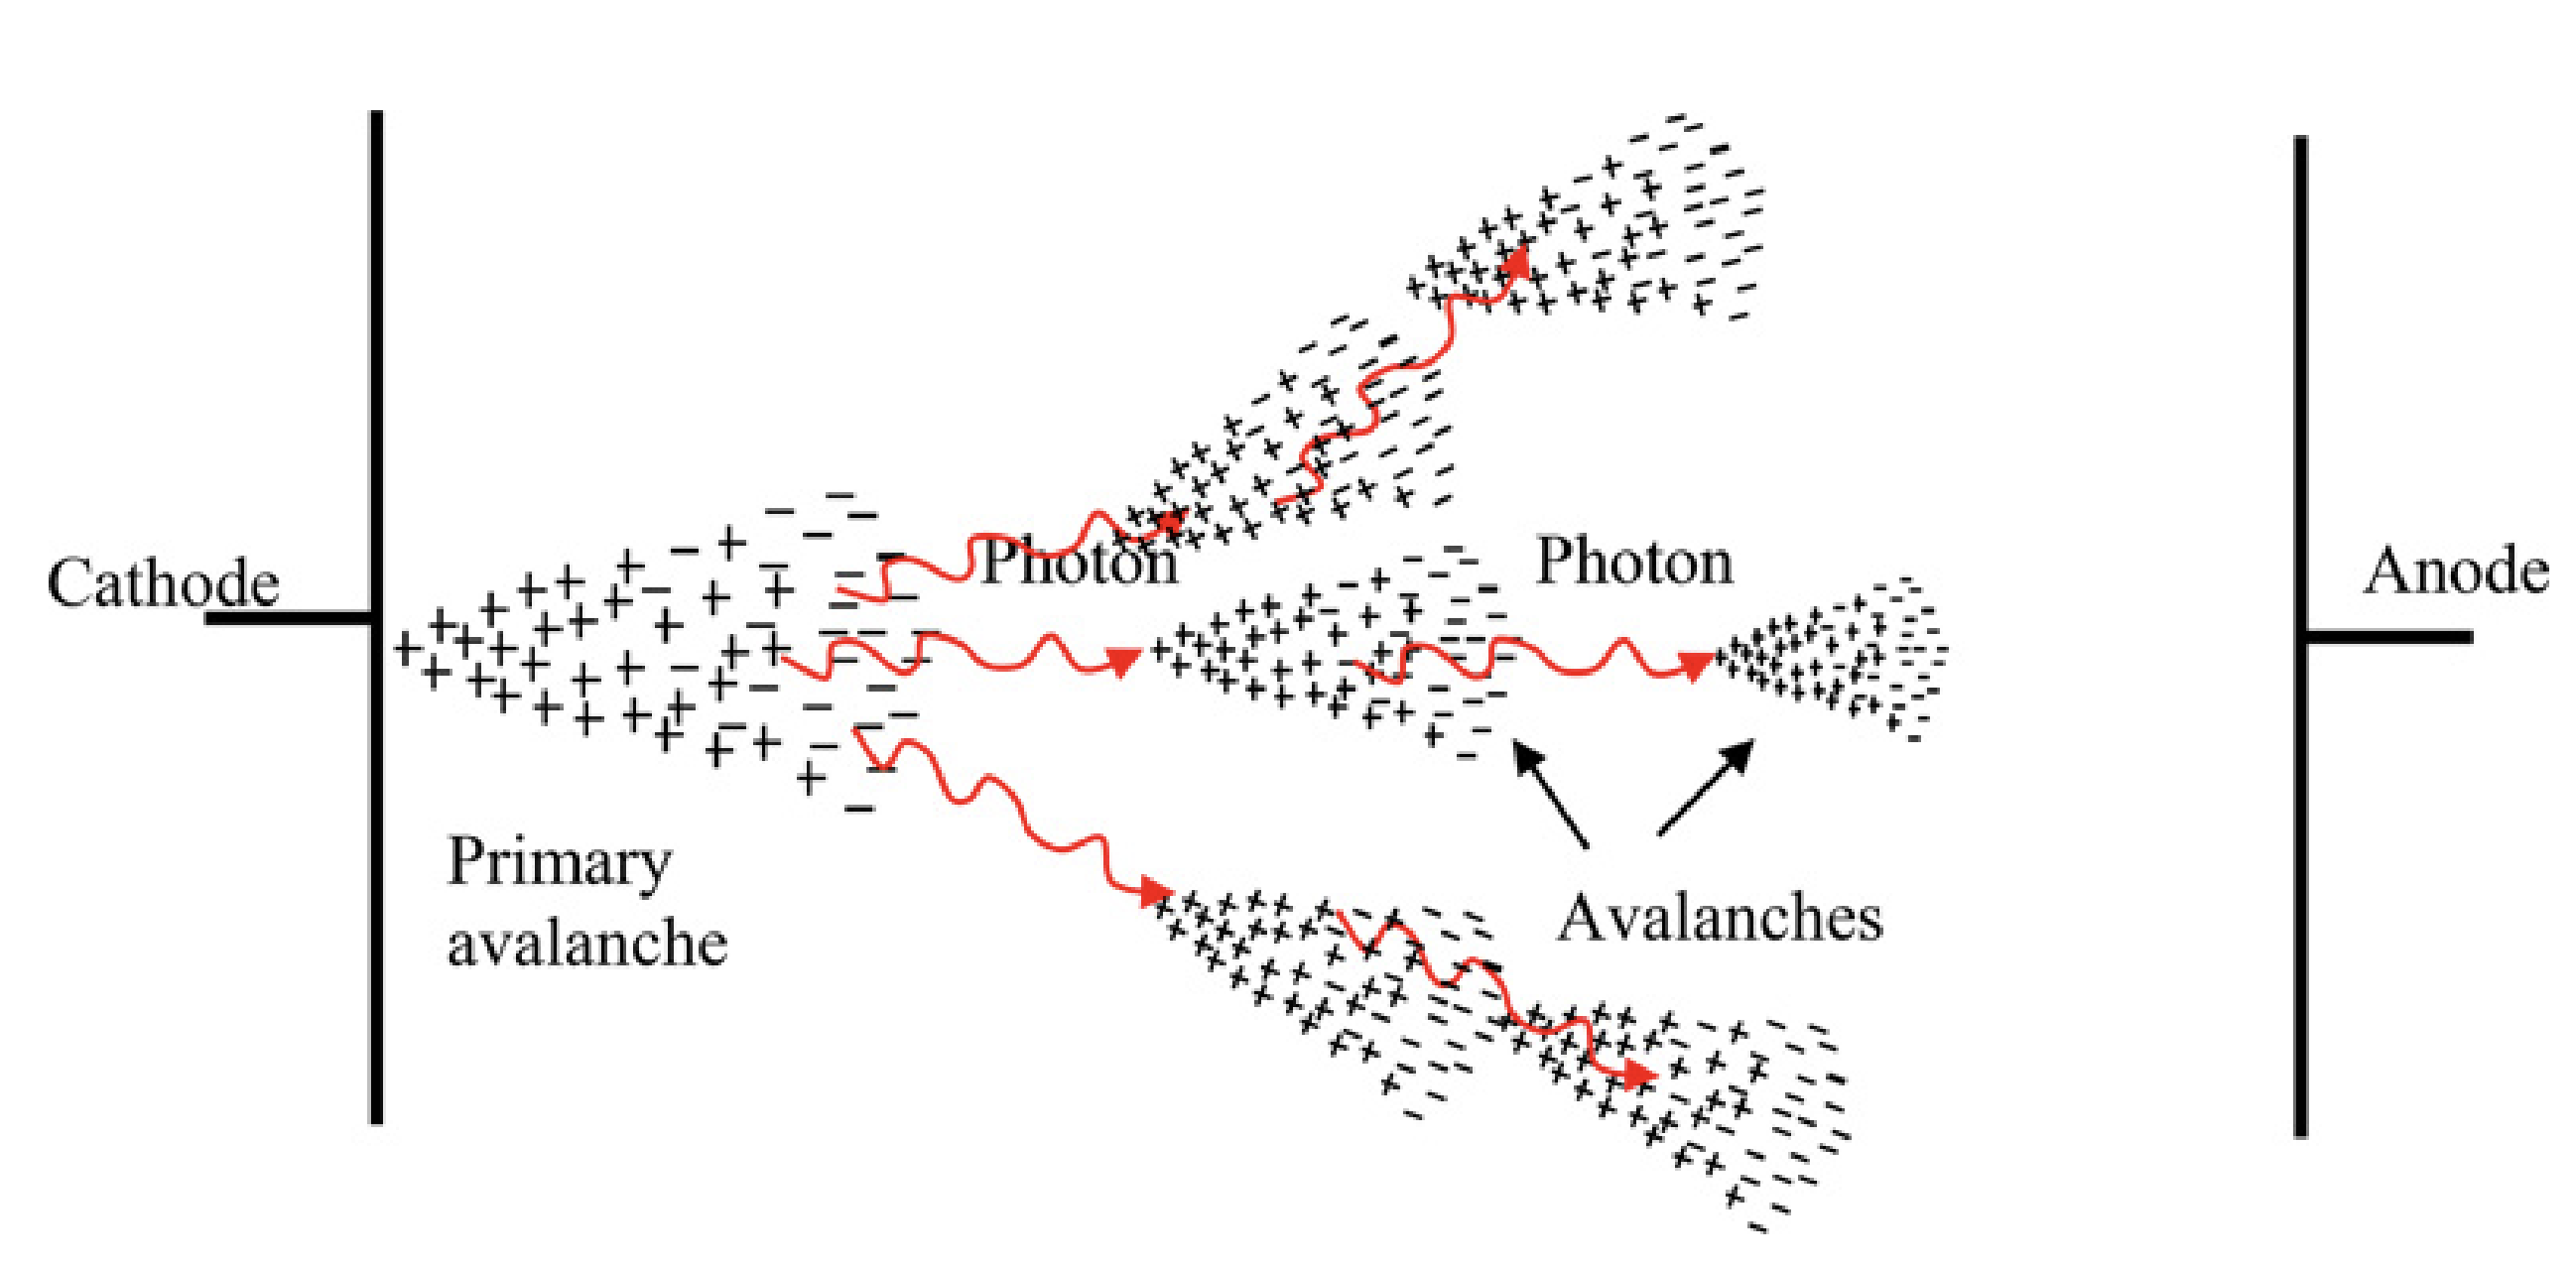
\includegraphics[width=0.5\textwidth,keepaspectratio]{figures_and_tables/rpc/streamer.png}
    \end{center}
    \caption{Streamer formation process. The distorted electric field around the high positive charge concentration enhances the ionization process, initiating secondary avalanches. Source:~\cite{livro_descarga}.}
    \label{streamer}
\end{figure}

A RPC where most of the charge multiplication process happens in the form of a streamer is said to be working in \textbf{Streamer Mode}. The advantage of the of the streamer mode is the high induced charge which is easily caught by non-sensitive readout electronics. On the other hand, the streamer mode, because of its highly associated charge, will have a impact in the rate capability of the detector (the local dead time will be higher).

Because of the high background environment of LHC, the CMS RPC operates in \textbf{Avalanche Mode}, where de discharge is highly quenched and very well localized. On the other hand, a very sensitive readout electronics is required to cope with the high rate demanded.

A good review of electrical discharge on gases can be found at~\cite{livro_descarga}.

\section{CMS Resistive Plate Chambers}

At CMS, the Resistive Plate Chamber are installed in both the barrel and endcap region, forming a redundant system with the DT (barrel) and CSC (endcap). As described in the CMS Muon Technical Design Report (Muon-TDR)~\cite{muon_tdr}, the RPC are composed of 423 Endcap chambers and 633 barrel chambers. Figure~\ref{picture_rpc} presents a picture of the CMS RPCs installed on station RE+4 of the Endcap.

\begin{figure}[h]
    \begin{center}
    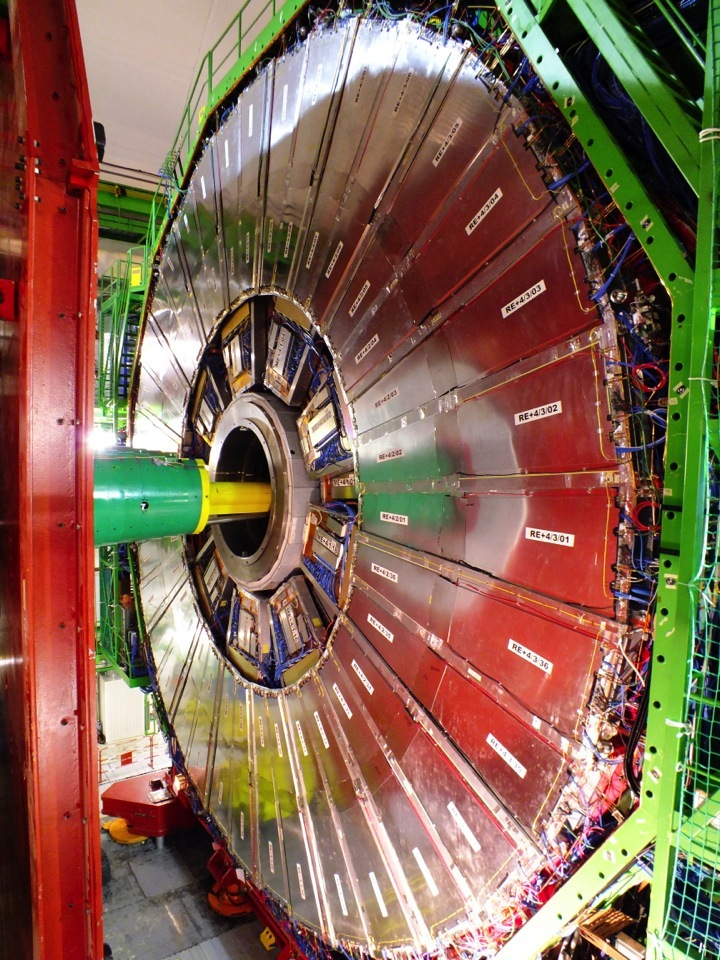
\includegraphics[width=0.5\textwidth,keepaspectratio]{figures_and_tables/rpc/picture_rpc.jpg}
    \end{center}
    \caption{RPC chamber on installed on station RE+4 of CMS Endcap. Source:~\cite{rpc_picture}.}
    \label{picture_rpc}
\end{figure}


Each chamber consists of two gas gaps (double gap), 2 mm tick each, made of Bakelite (phenolic resin) with bulk resistivity of $10^{10}$ - $10^{11}$ $\Omega m$. The choice of the bulk resistivity of the electrode has high impact on the rate capability of the detector.

Each gap has its external surface is coated with a thin layer of graphite paint, which acts as conductive material, distributing the applied high-voltage (HV). On top of the graphite a PET film is used for isolation. A sheet of copper strips is sandwiched between the gaps. Everything is wrapped in aluminum case.

The double gap configuration increases the efficiency of the chamber, since the signal is picked up from the OR combination of the two gaps. A chamber with only one gap working, looses around 15\% of efficiency, even though, this can be recovered by increasing the HV applied during operation mode (working point - WP).

A characteristic that differentiate the CMS RPC  from from previous RPC application in HEP is the operation mode. A RPC at CMS, operates in avalanche mode, while previous experiments used the streamer mode. Both modes are related to the applied HV, in commitment with the strength of the generated signal, and are capable of generate a well localized signal, which can be picked up by the readout electronics, but the avalanche mode offer a higher rate capability around 1 kHZ/$cm^2$, while the streamer mode goes up to 100 HZ/$cm^2$. The high rate capability is a key factor in order to cope with requirements of the LHC luminosity, specially in the high background regions.

Besides the rate capability, the key factors that driven the CMS RPC design were:  high efficiency ($> 95\%$), low cluster size ($> 2$) for better spatial resolution (this reflects in the momentum resolution) and good timing in order to do the readout of the signal within the 25 ns of a LHC bunch cross (BX) and provide it to the CMS trigger system. These requirements have implications in the choice of material, dimensions, electronics and gas mixture.

In the barrel, along the radial direction, there are 4 muon layers (called stations), MB1 to MB4. MB1 and MB2 is composed of a DT chamber sandwiched between two RPC chambers (RB1 and RB2) with rectangular shape. The stations MB3 and MB4 have only one RPC (RB3 and RB4) are composed by two RPC chambers (named - and + chambers with the increase of $\phi$) attached to one DT chamber, except in sector 9 and 11, where there is only one RPC. RE4, sector 10 is a special case, since it is composed of four chambers (--, -, + and ++). These stations are replicated along the z direction in five different wheels of the CMS (W-2, W-1, W0, W+1 and W+2) and in twelve azimuthally distributed sectors (S1 to S12). Figure~\ref{fig:barrel_rphi_rz} show the different barrel stations and wheel.


\begin{figure}[h]
\begin{center}
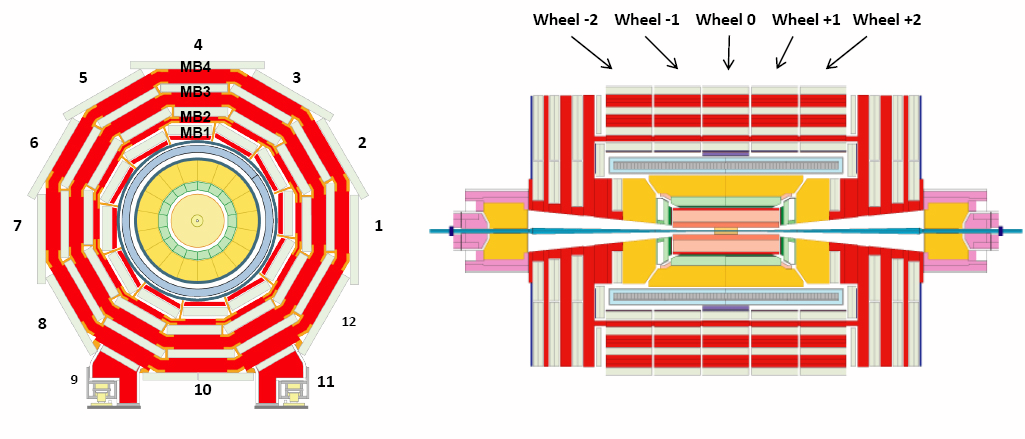
\includegraphics[width=1.0\textwidth,keepaspectratio]{figures_and_tables/rpc/barrel_rphi_rz.png}
\end{center}
\caption{R-$\phi$ (left) and R-Z (right) projections of the barrel Muon System.}\label{fig:barrel_rphi_rz}
\end{figure}


In the endcap, the RPC chambers have a trapezoidal shape and are distributed in four disks (or stations) each side (RE$\pm4$, RE$\pm3$, RE$\pm2$, RE$\pm1$), each one with 72 chambers. CMS split up its disks in 3 rings, along the radial direction, and 36 sector in the azimuthal angle. RPCs are present in the two outer rings (R2 and R3), in all 36 sectors. The RE$\pm4$ are special cases, since these chambers were installed only in 2014, a design choice was made the mechanically attached R2 and R3 chambers, each sector, in what is called, a super-module. Figure~\ref{fig:endcap_rz} show the different endcap disks.

\begin{figure}[h]
\begin{center}
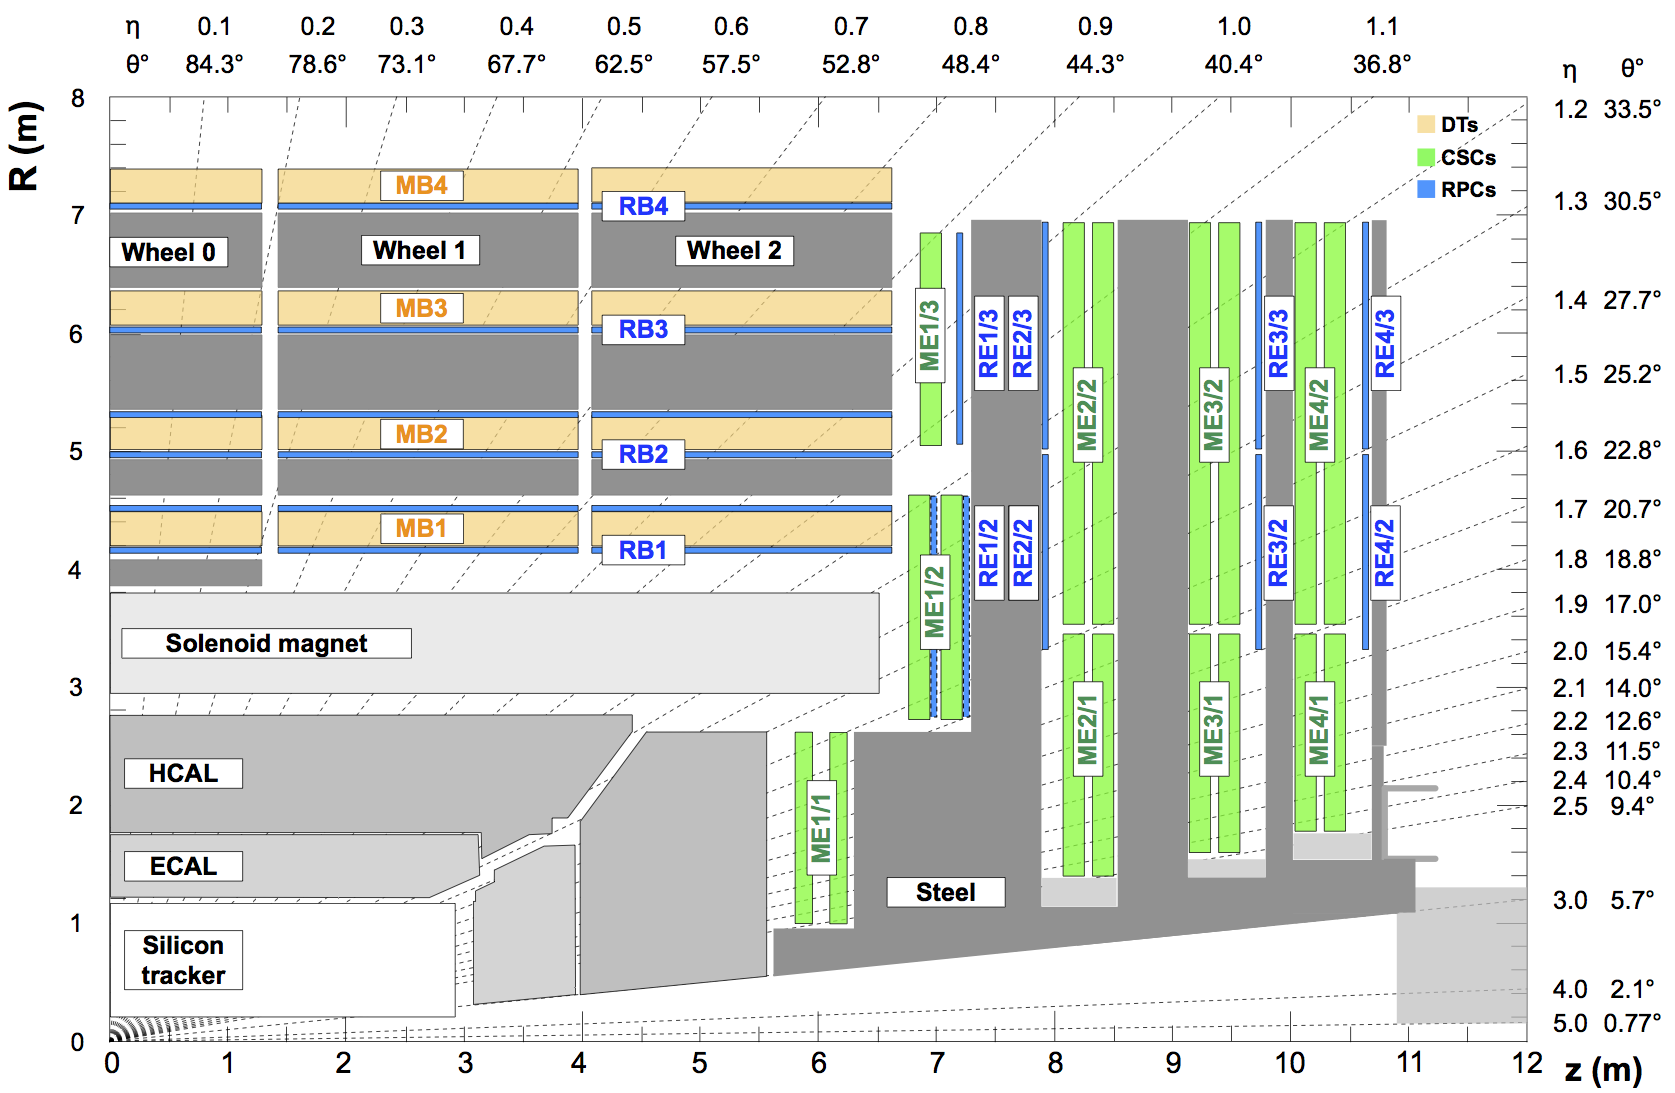
\includegraphics[width=1.0\textwidth,keepaspectratio]{figures_and_tables/rpc/endcap_rz.png}
\end{center}
\caption{R-Z projections of the endcap Muon System (positive Z side). This is the same configuration for the 36 $\phi$ sectors.}\label{fig:endcap_rz}
\end{figure}

The length of the strips is chosen, for both barrel and endcap, in such a way to control the area of each strip, in order to reduce the fake muons, due to random coincidence. This has to do with the time-of-flight and signal propagation along the strip. In the barrel, each chamber readout is divided in two regions (rolls), called forward and backward (along increasing $|\eta|$)~\footnote{Some chamber are divided in three rolls, forward, middle and backward, for trigger propose.}. In the endcap, the strips are divided in 3 regions, called partitions A, B and C (from inside the detector to outside).


The gas mixture used in the CMS RPCs is composed by C2H2F4 (Freon R-134a, tetrafluoroethane), C4H10 (isobutane), SF6 (sulphur hexafluoride) (95.2 : 4.5 : 0.3 ratio) and with controlled humidity of 40\% at 20-22 $^{\circ}$C. The Freon is used to enhance the ionization and charge multiplication that characterizes the avalanche, while the isobutane is introduced for quenching proposes, in order to reduce the secondary ionizations that could lead to formation of streamers and the SF6 is used to reduce the electron background. The choice of Freon over other gases, i.e. argon-based and helium-based, was motivated by previous studies~\cite{gas_mixture_BERNARDINI1995428,gas_mixture_Gorini}.


Since its R\&D, the RPC have shown good performance over aging. This is even historical over previous RPC experiments~\cite{Bressi:1987kg,Ge:2014tea,Abbrescia:1993xy,Antoniazzi:1992dg,DiCiaccio:1992di,deAsmundis:1995dq,Boutigny:1995ib}. Even the most recent studies of aging, taking into account future LHC conditions (High-Luminosity LHC - HL-LHC) plus a safety margin of 3 times the expected background (600 HZ/$cm^2$) have shown good aging hardness~\cite{andrea_rpc_2018}.

\subsection{Performance}

The RPCs, for the CMS experiment, contribute mainly with triggering inputs, due to its very good time resolution. The important parameters which are monitored to evaluate the RPC performance are the efficiency and cluster size. The former is related to the ratio of the registered hits over the number of muons that passed through the chamber, while the former one is the number adjacent strip (minimal readout unit) that were fired (activated) per hit. Figures~\ref{eff_run2} and \ref{cls_run2} present the historical distribution of efficiency and cluster size as a function of the integrated luminosity collect during Run2.

\begin{figure}[htbp]
    \centering
    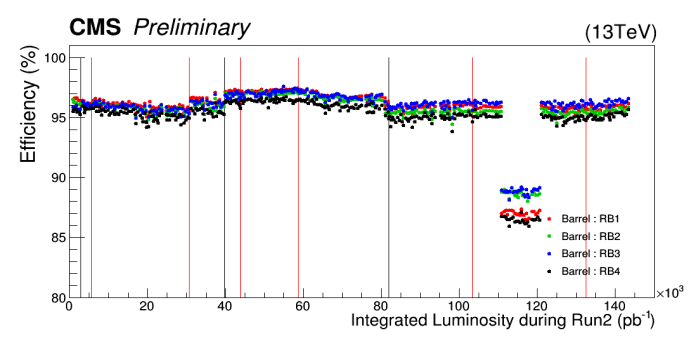
\includegraphics[width=0.47\textwidth,keepaspectratio]{figures_and_tables/rpc/performance/barrel_eff_vs_intL.png}
    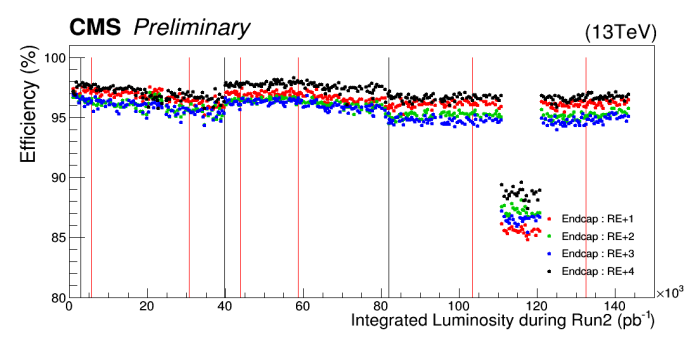
\includegraphics[width=0.47\textwidth,keepaspectratio]{figures_and_tables/rpc/performance/endcap_eff_vs_intL.png}
    \caption{RPC efficiencies (per chamber) over Run2 Integrated Luminosity for Barrel (left) and Endcap (right). Red lines indicates technical stops (TS) while grey ones indicates Year-End-Technical stops (YETS). The drop in the efficiency around 110 $pb^{-1}$ is related to a known operation mistake. Source:~\cite{rpc_run2_performance}.}
    \label{eff_run2}
\end{figure}

\begin{figure}[htbp]
    \centering
    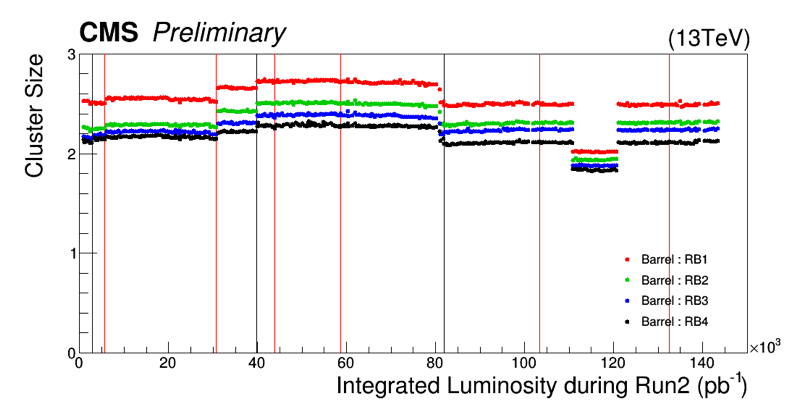
\includegraphics[width=0.47\textwidth,keepaspectratio]{figures_and_tables/rpc/performance/barrel_cls_vs_intL.png}
    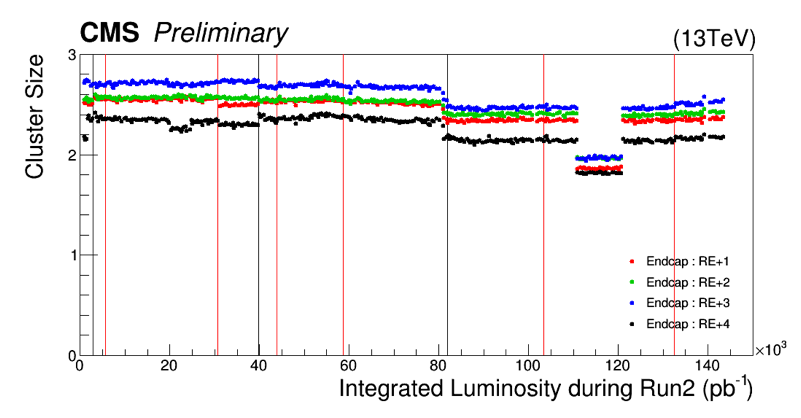
\includegraphics[width=0.47\textwidth,keepaspectratio]{figures_and_tables/rpc/performance/endcap_cls_vs_intL.png}
    \caption{RPC cluster size (CLS - per chamber) over Run2 Integrated Luminosity for Barrel (left) and Endcap (right). Red lines indicates technical stops (TS) while grey ones indicates Year-End-Technical stops (YETS). The drop in the cluster size around 110 $pb^{-1}$ is related to a known operation mistake. Source:~\cite{rpc_run2_performance}.}
    \label{cls_run2}
\end{figure}

In general, the RPC system operates with efficiency above 95\% and cluster size smaller than 3 (a good parameter established during the design phase). The importance of the efficiency is a less complicated concept to catch, on the other hand, the cluster size might not be so straight forward. The optimal regime of RPCs operation at CMS is the avalanche mode, in which the electrical discharge is constrained in a millimeter level size region. Another operation mode is the streamer mode, in which the initial discharge might trigger secondary ones, e.g. by the emission of unquenched photons. A streamer discharge is capable of fire neighbor strips, increasing the cluster size. Operating in avalanche mode is fundamental to keep the RPCs capable of dealing with the high background environment of CMS. 

To keep the mean cluster size under control ($< 3$) is important to guarantees enough spatial resolution for the measurements (the geometrical position of a hit is the midpoint of the cluster) and ensures that the system has enough rate capability to operate, since a RPC with a high sensitive front-end electronics (necessary for the avalanche mode operation) could be degraded by pileup of dead time on many channels, including electronics noise, streamers, darks counts and other sources of background.

A third important parameter to be measured and controlled in a RPC system, under the LHC conditions, is the current due to the high voltage applied. This current is known to be proportional to the total charge released in each electrical discharges and to the hit rate on the chamber. The voltage applied is divided, as in a series circuit, between the electrodes and the gap. At increasing background, the current also increases and, since the applied voltage is constant, the voltage across the gap is reduced in favor of the voltage across the electrodes. This reduction of effective voltage on the gas, might have an impact on its gain, imposing a reduction on the detector sensitivity.

Figure~\ref{cms_run2_currents} presents the ohmic currents~\footnote{Current at 6500 V, which is below the typical working point of a CMS RPC (around 9500 V). In this region, no charge multiplication effect take place and chamber current is governed only by Ohm's Law.} in different regions of the detector, from $16^{th}$ of April, 2018 to $2^{nd}$ of December, 2018. It is clear how the stations subjected to higher background (RE$\pm$4 - 40 $Hz/cm^2$) are subjected to a degrading factor that increases with the luminosity (background rate) and decreases when the detector is powered off. This effect is supposed to be related with the Hydrogen Fluoride (HF) production inside the gap, due to the electrical discharges. HF is a conductivity molecule, which can potentially attach to the internal surface of the gap, reducing the overall resistivity. The HF production can be controlled by properly tunning the gas flow as a function of the background that the chamber is subjected. HF concentration can also lead to permanent degradation of the gap, due to its chemical properties. Keeping the currents levels as low as possible is important for aging proposes. 

\begin{figure}[htbp]
    \centering
    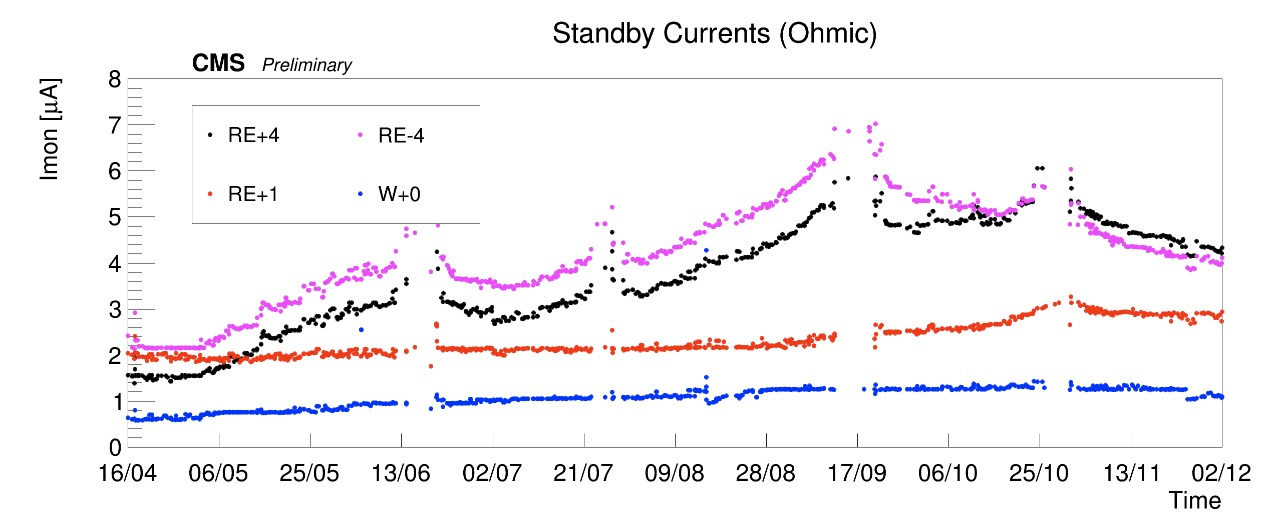
\includegraphics[width=0.9\textwidth,keepaspectratio]{figures_and_tables/rpc/performance/ohmic_current_run2.png}
    \caption{Ohmic current history of W+0, RE+1, RE+4 and RE-4. The blank regions, from time to time, corresponds to technical stops (TS), when the detector is off. Source:~\cite{rpc_run2_performance}.}
    \label{cms_run2_currents}
\end{figure}

A review of the RPC performance during Run2 can be found at~\cite{rpc_run2_performance}.

\section{Contribution to the CMS RPC project}

During the curse of this study, a head collaboration of our research group and the CMS RPC project was established. Many contributions were given to the project as part of the graduation as a experimental particle physicist, with focus on getting acquaintance with a subsystem technology and give a meaningful collaboration to the detector operation.  Those are considered by the community important steps on the student graduation.

Bellow it is described the contributions given to the CMS RPC project.

\subsection{RPC Operation - Shifts and Data Certification}

The first activities done for the CMS RPC project were shifts for data certification of data taken. This certification is done by specialized people for different CMS subsystems and physics objects groups~\footnote{Groups of reconstruction and performance experts for different high-level reconstructed objects from CMS, i.e. muons, taus, jets/MET, electrons/photons}. 
 
This certification is done in order to ensure the quality of the date recorded based on the well functionality of each system during the data taking and the reconstruction of the physics objects in the expected matter. A certain collection of data (run) is said certificate when all subsystems and object experts agrees on this.

Figure~\ref{lumi} shows, as an example of the luminosity delivered by the LHC, recorded one by CMS and the certified (validated), from the 22nd of April, 2016 to the 27th of October, 2016. Only certified data is available for physics analysis.

Shifts are a continuous weekly activity (specially during the data taking period), performed in a weekly basis, in order to ensure the availability of certified data, as soon as possible.  

\begin{figure}[htbp]
    \centering
    \begin{subfigure}[b]{0.6\textwidth}
        \centering
        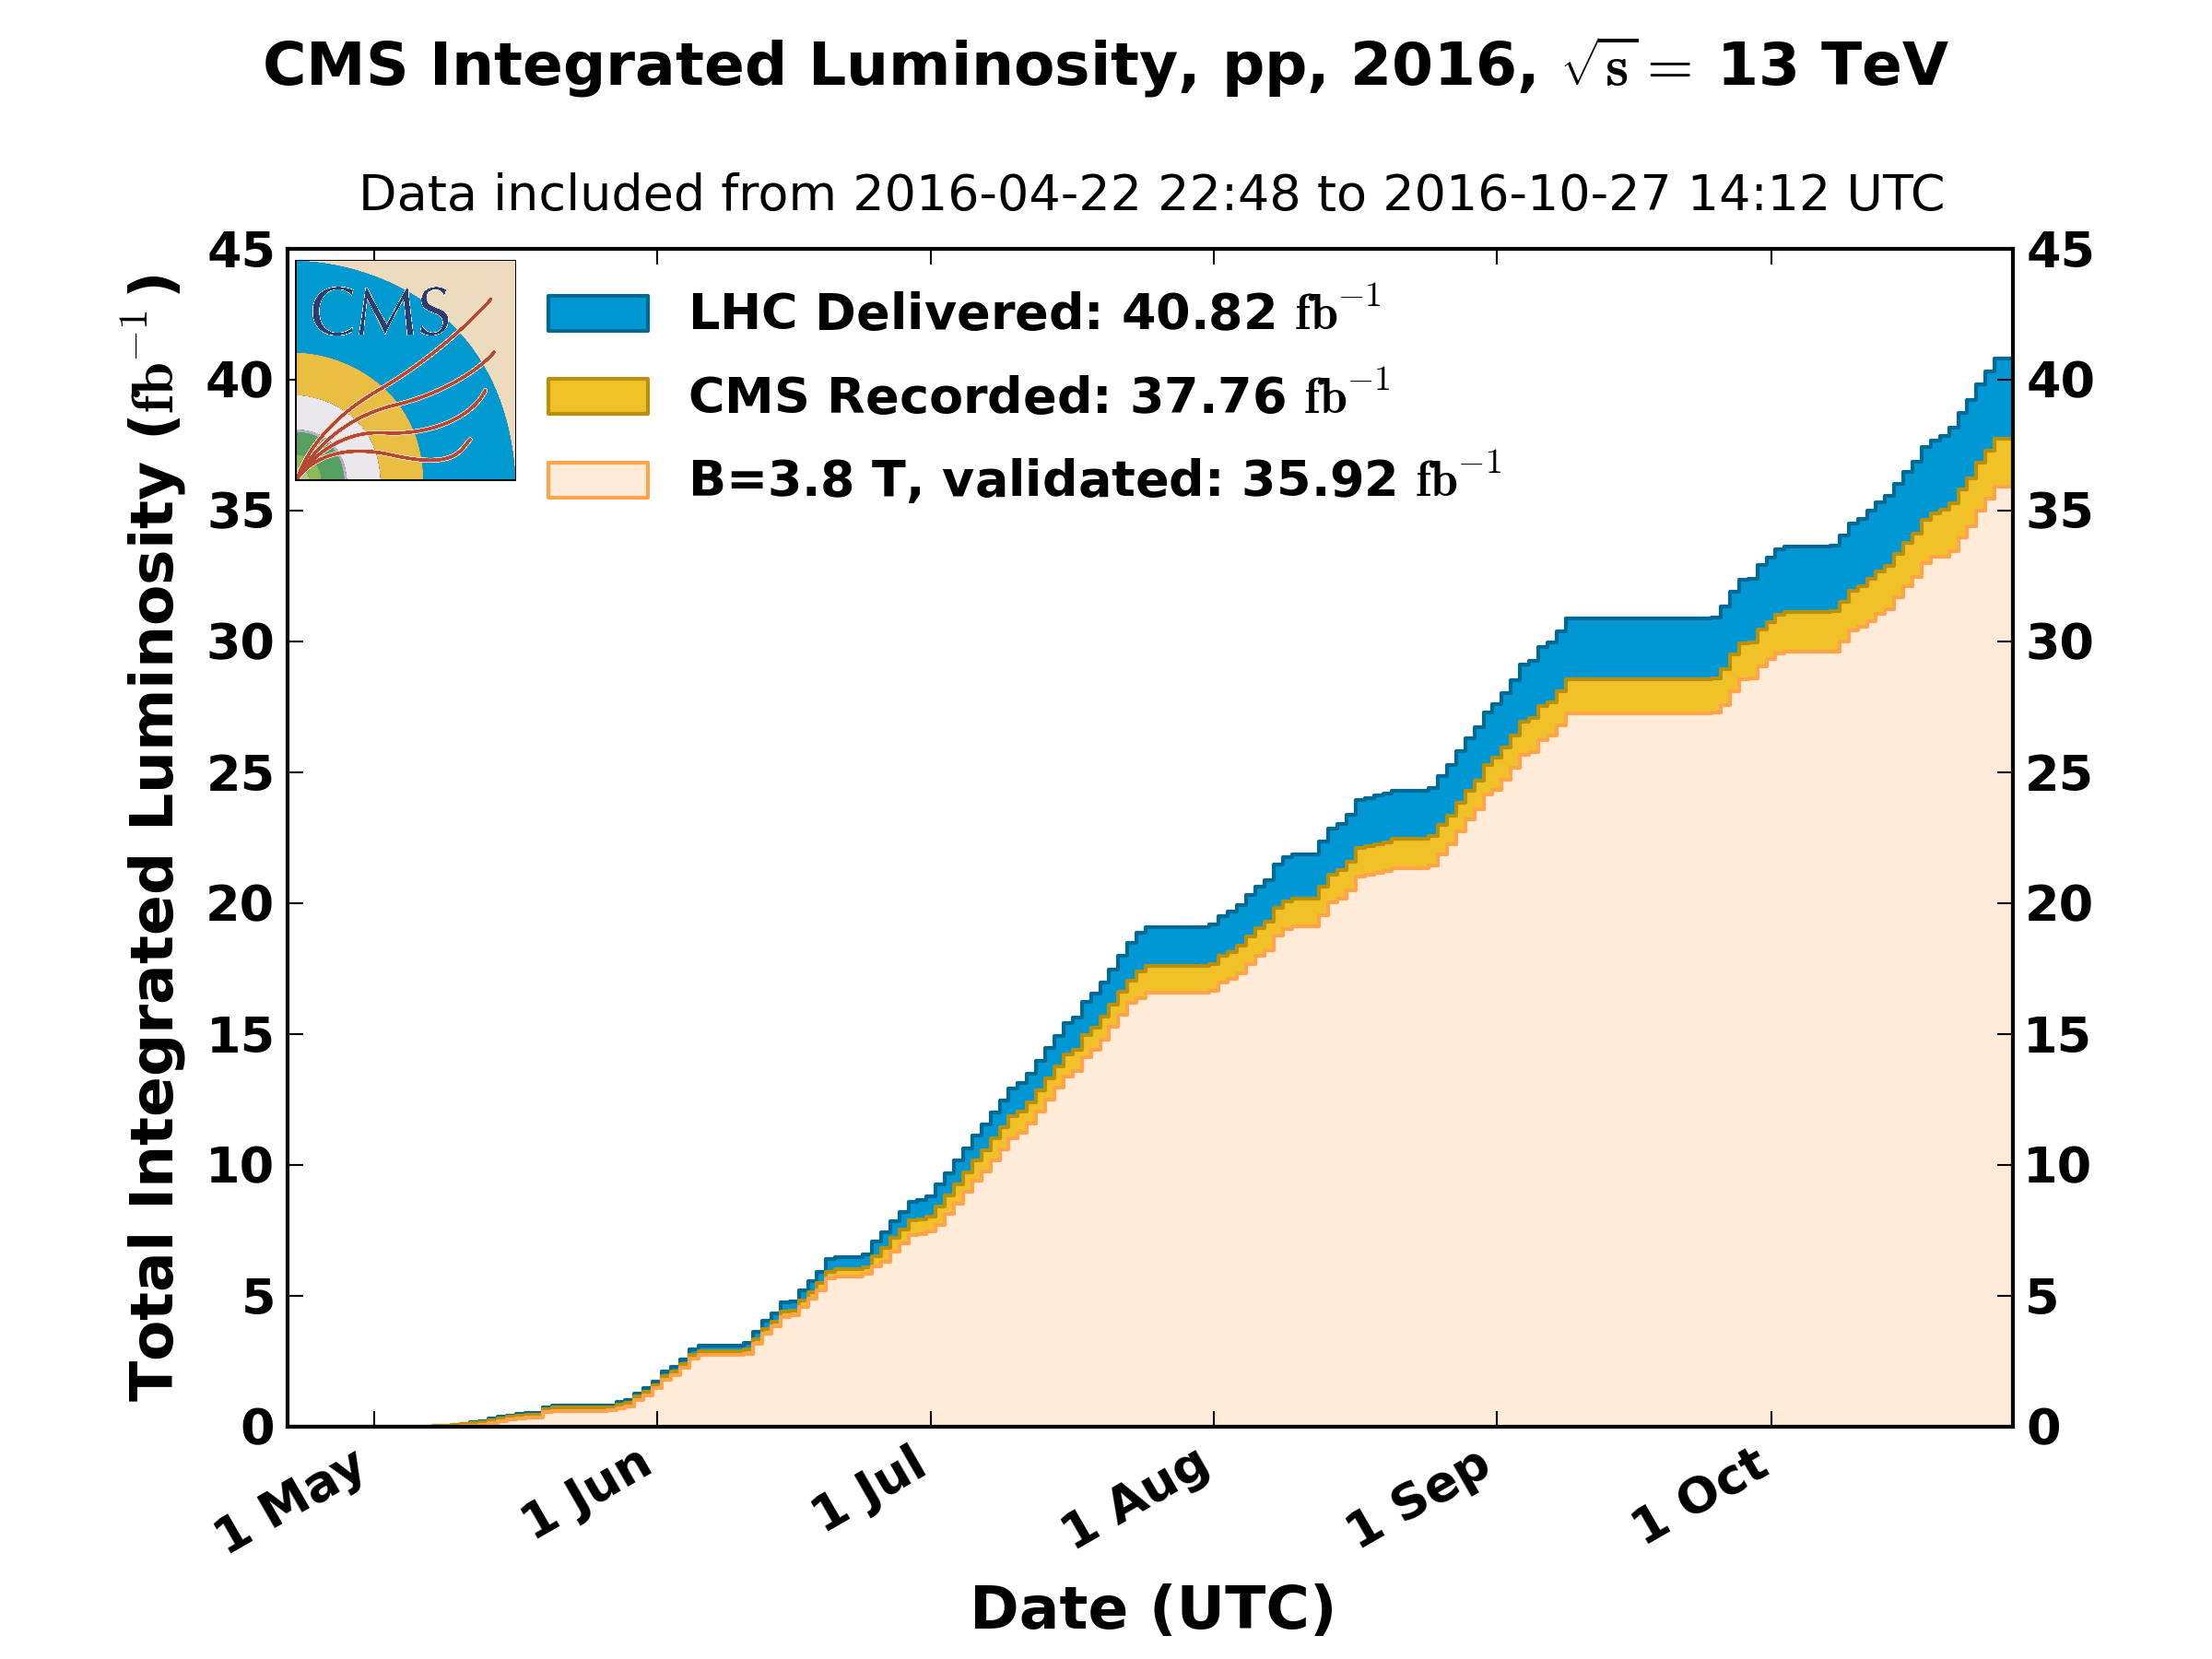
\includegraphics[width=\textwidth]{figures_and_tables/rpc/lumi_plot.png}  
        \caption{}
        % \label{fig:sub-second}
    \end{subfigure}
    \hfill
    \begin{subfigure}[b]{0.35\textwidth}
        \centering
        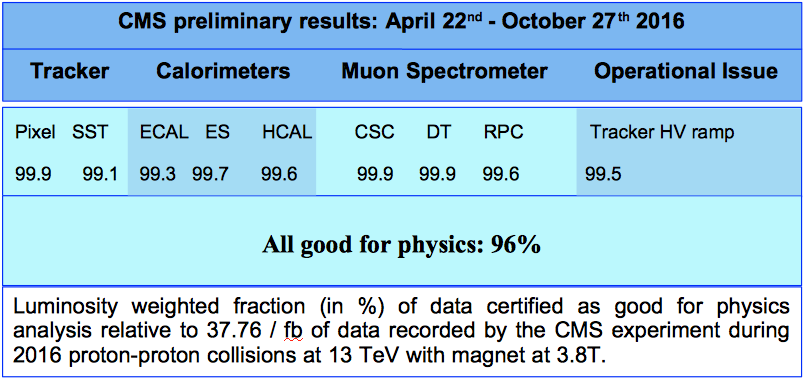
\includegraphics[width=\textwidth]{figures_and_tables/rpc/lumi_table.png}  
        \caption{}
        % \label{fig:sub-second}
    \end{subfigure}
    \caption{(a) Luminosity delivered by the LHC, recorded one by CMS and the certified (validated), from the 22nd of April, 2016 to the 27th of October, 2016. (b) Efficiency of the certification process for each subsystem, from the 22nd of April, 2016 to the 27th of October, 2016. Total CMS efficiency is above 90\%. Source:~\cite{certification}}%
    \label{lumi}%
\end{figure}

\section{RPC Online Software}

On what concerns the Online Software (OS) of the CMS RPC system, the main contribution given was the upgrade of the Trigger Supervisor libraries.

The Trigger Supervisor is a web-based software, which run over the xDAQ backend and provides, through a modules organized in a tree system, called cells, a standard interface for the operation and monitoring of different system at CMS. In principle only systems which contribute directly to the L1 trigger should have a Trigger Supervisor implementation. This was the case for the  RPC during the Run1. Since Run2, RPC contributes to the trigger indirectly, by providing data to the muon processors (CPPF, OMTF and TwinMux). The Trigger Supervisor implementation is a legacy from that period.

Each subsystem is responsible for its own implementation of the Trigger Supervisor, based on the functionalities that it wants to have (requirements). The xDAQ~\cite{xdaq} is a middleware, developed by CERN and widely used at CMS, as a tool for control and monitoring of data acquisition system in a distributed environment. It is capable of providing a software layer for direct access of hardware functionalities and monitoring.

The upgrade made (figure~\ref{ts_upgrade}), consists in upgrade the higher level of the RPC online software. In summary, up to 2017, the online software, was using Scientific Linux 6 as operational system, which executed xDAQ 12, in turn, servers as backend for Trigger Supervisor 2. A upgrade of the operational system to Centos 7, demanded the upgrade to xDAQ 14. On top of that, Trigger Supervisor 2 would not work and had to be updated to Trigger Supervisor 5 in order to be functional in 2018.

\begin{figure}[h]
\begin{center}
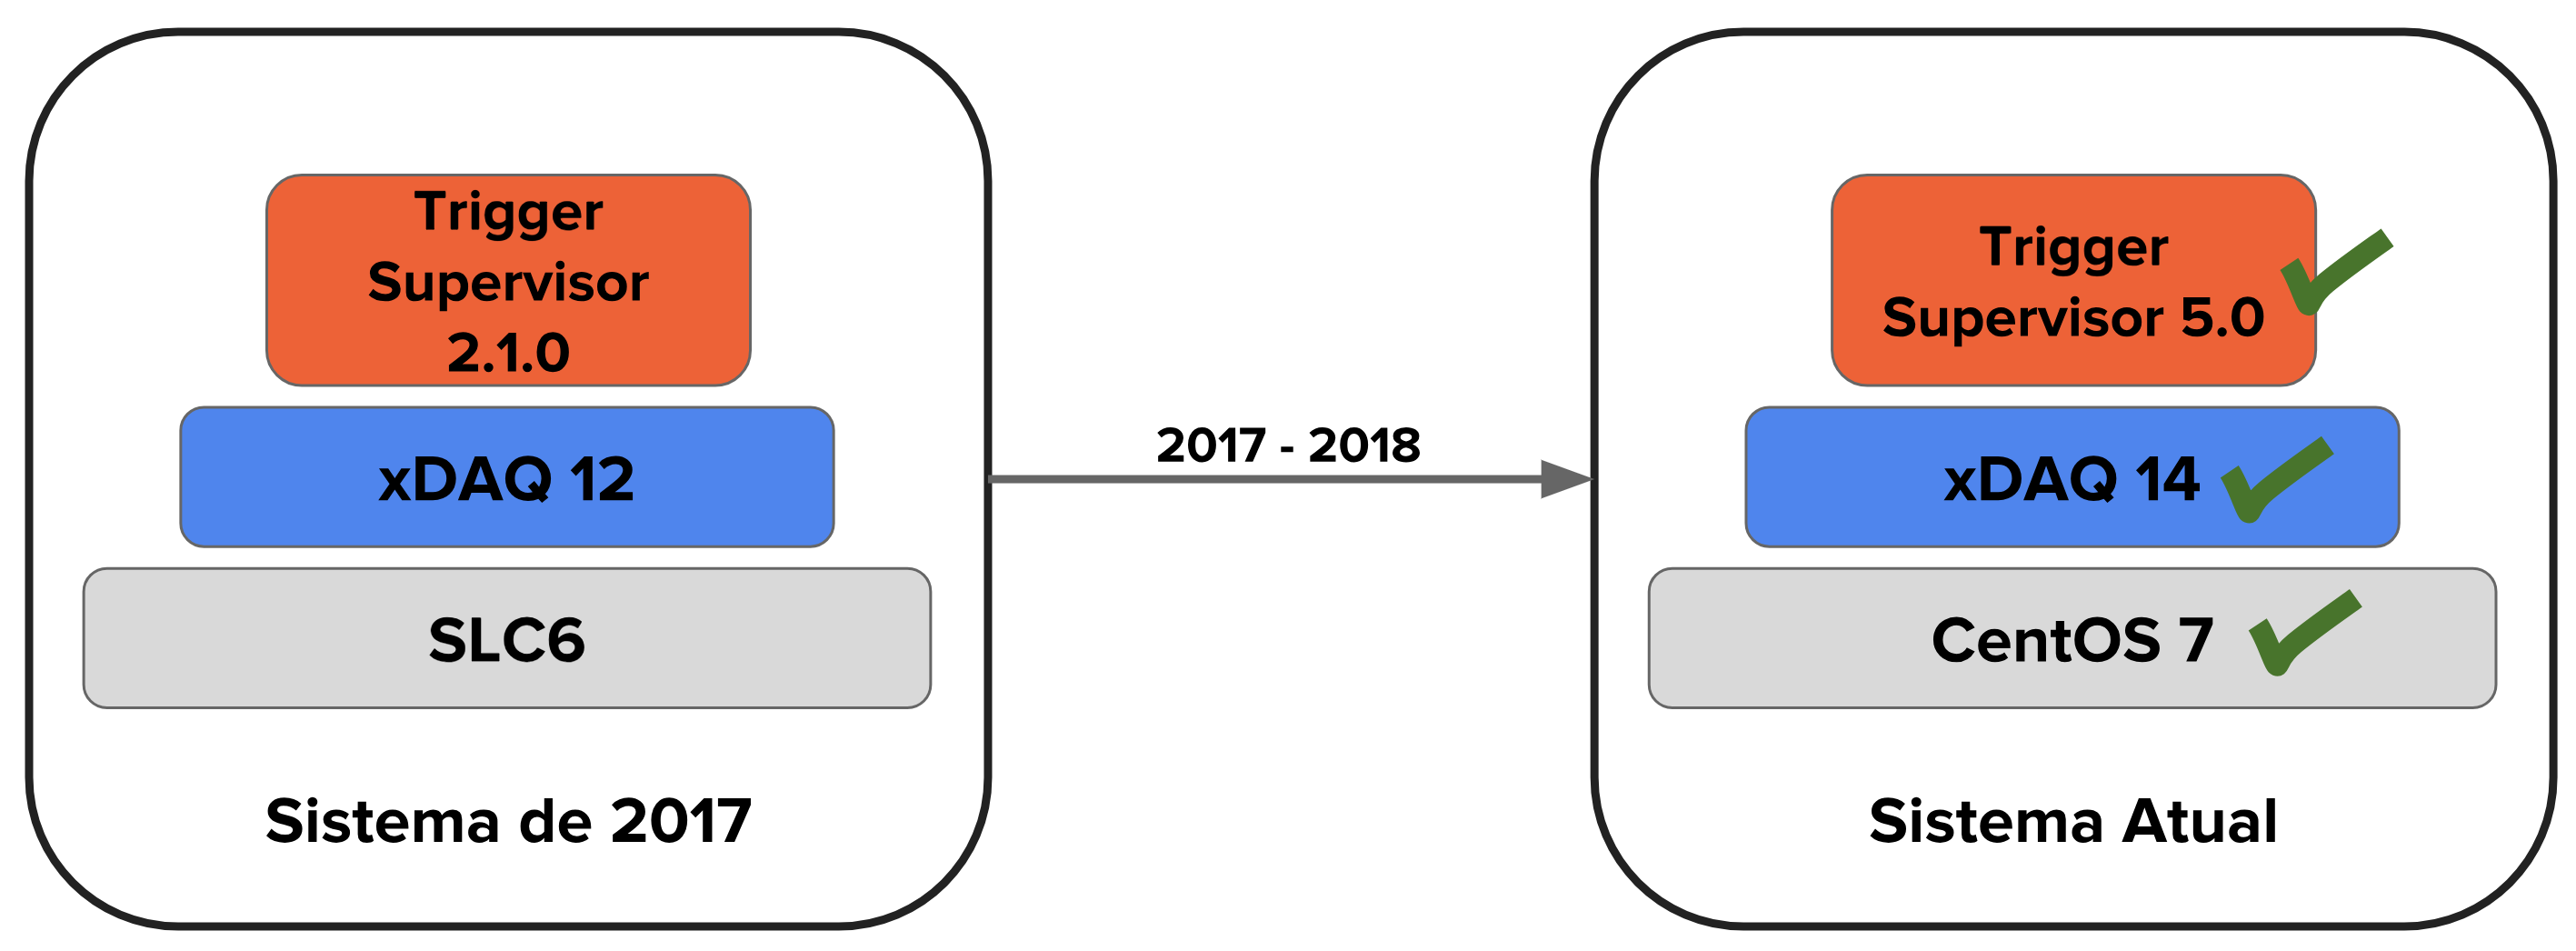
\includegraphics[width=0.8\textwidth,keepaspectratio]{figures_and_tables/rpc/ts_upgrade.png}
\end{center}
\caption{Upgrade of the RPC online software.}\label{ts_upgrade}
\end{figure}

Between versions 2 and 5 of Trigger Supervisor, part of the source-code had to be reworked, keep the majority of the code structures. Most of the changes were made in the front-end of the system. The standard JavaScript library Dojo~\cite{dojo}, used in version2, was deprecated in favor of Google's Polymer\cite{polymer}. The main reason for this change was to isolate C++ code from HTML, which was impossible with Dojo. This implied to rewrite all the screen of the RPC Trigger Supervisor implementation, as in figure~\ref{ts_view}.

The upgrade  was done in time to ensure the control and operation of the RPC for 2018 data taking.

\begin{figure}[h]
\begin{center}
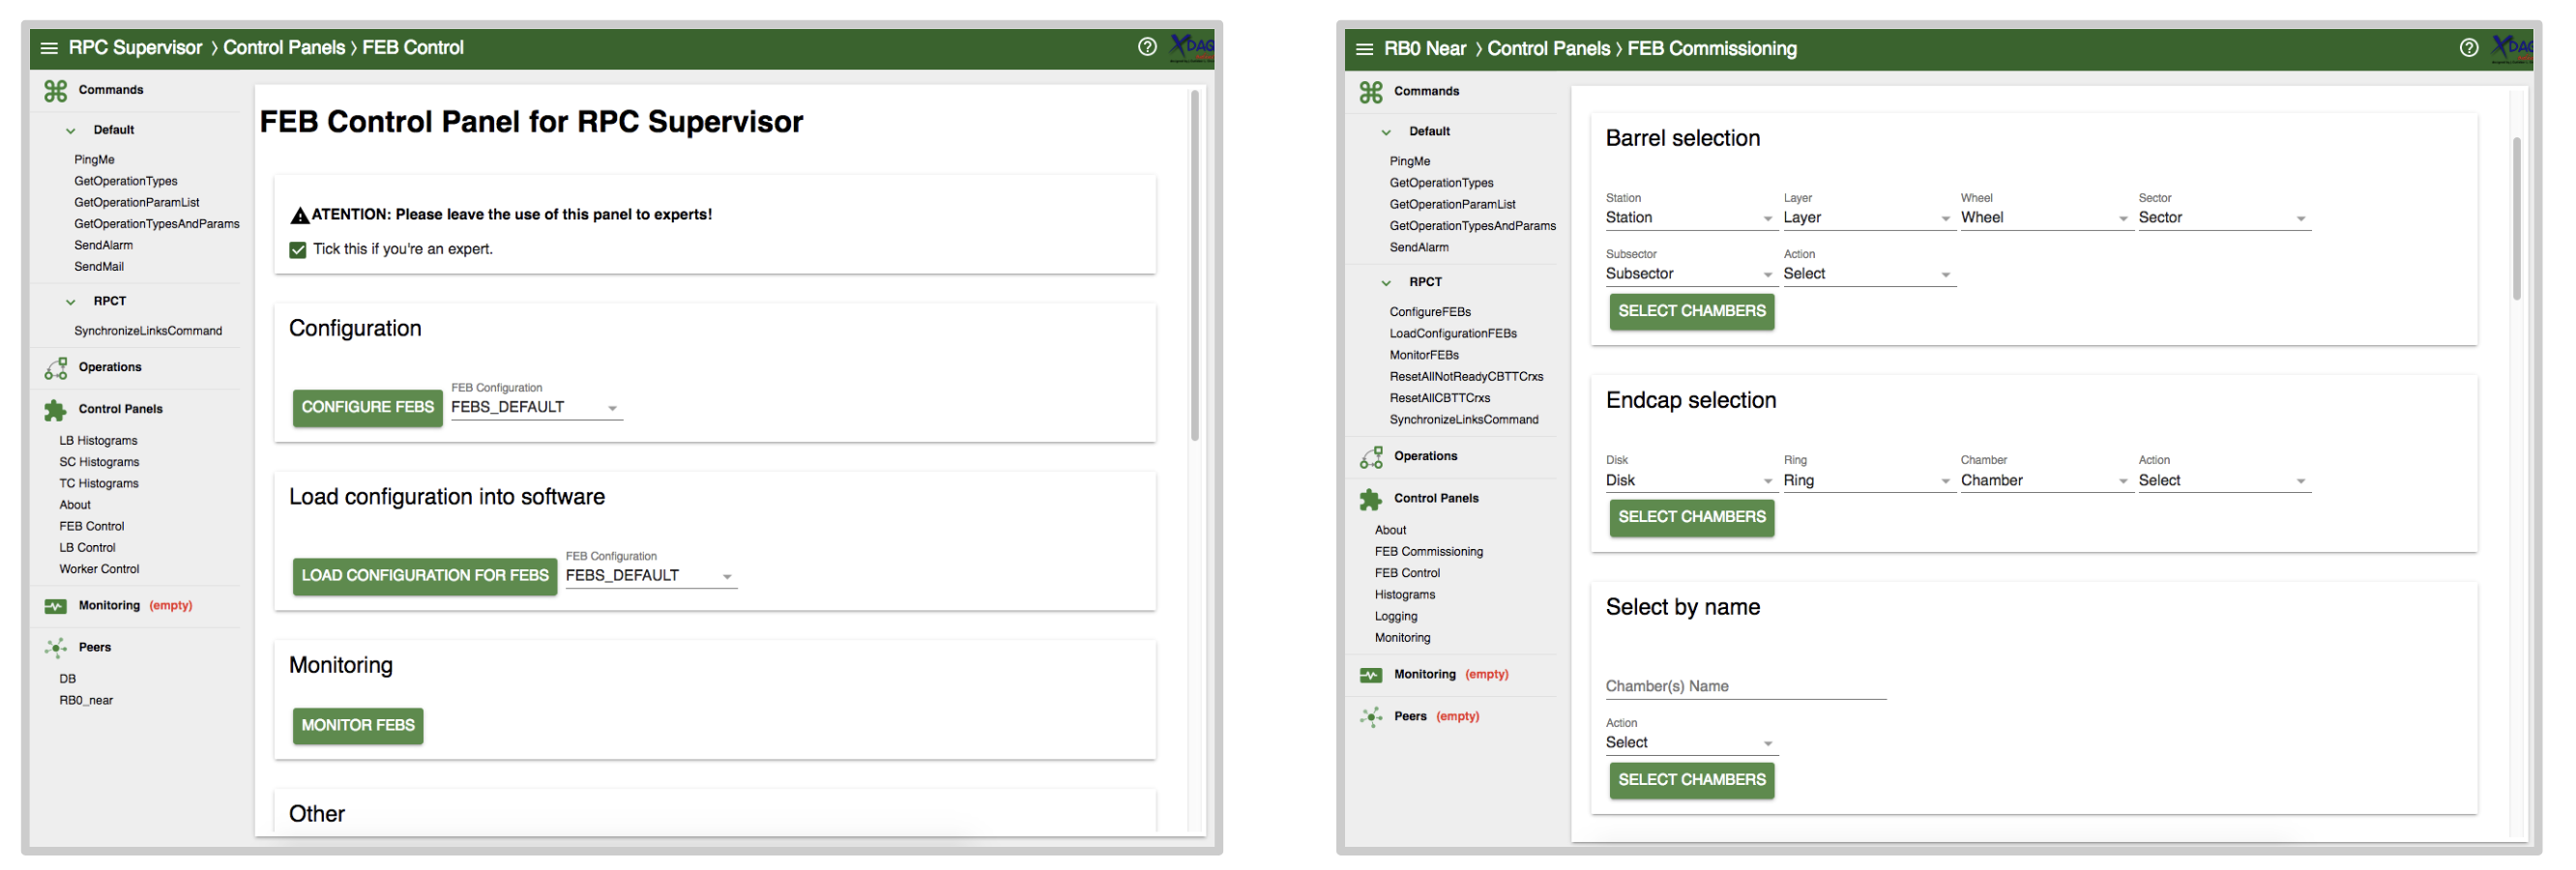
\includegraphics[width=0.95\textwidth,keepaspectratio]{figures_and_tables/rpc/ts_view.png}
\end{center}
\caption{Example of the updated screens, using Trigger Supervisor 5.}\label{ts_view}
\end{figure}


\subsection{iRPC R\&D}

For the next 4 year of CMS activities it is foreseen  the upgrade of the the Muon Systems~\cite{muon_tdr}. These upgrades are planed in order to extend the pseudorapidity coverage ($\eta$) and to guarantee the operation conditions of the present system in the HL-LHC (High Luminosity LHC) era. The RPC (Resistive Plate Chambers)~\cite{muon_tdr} subsystem, it will have maintenance of the present chambers and installation of new chambers in the region of $|\eta| < 1,8$ para $|\eta| < 2,4$~\cite{pedrazamorales2018rpc}. These new chambers (iRPC) will be added in the most internal part of the muon spectrometer, RE3/1 e RE4/1, as in Figure~\ref{muons_eta}.

\begin{figure}[h]
\begin{center}
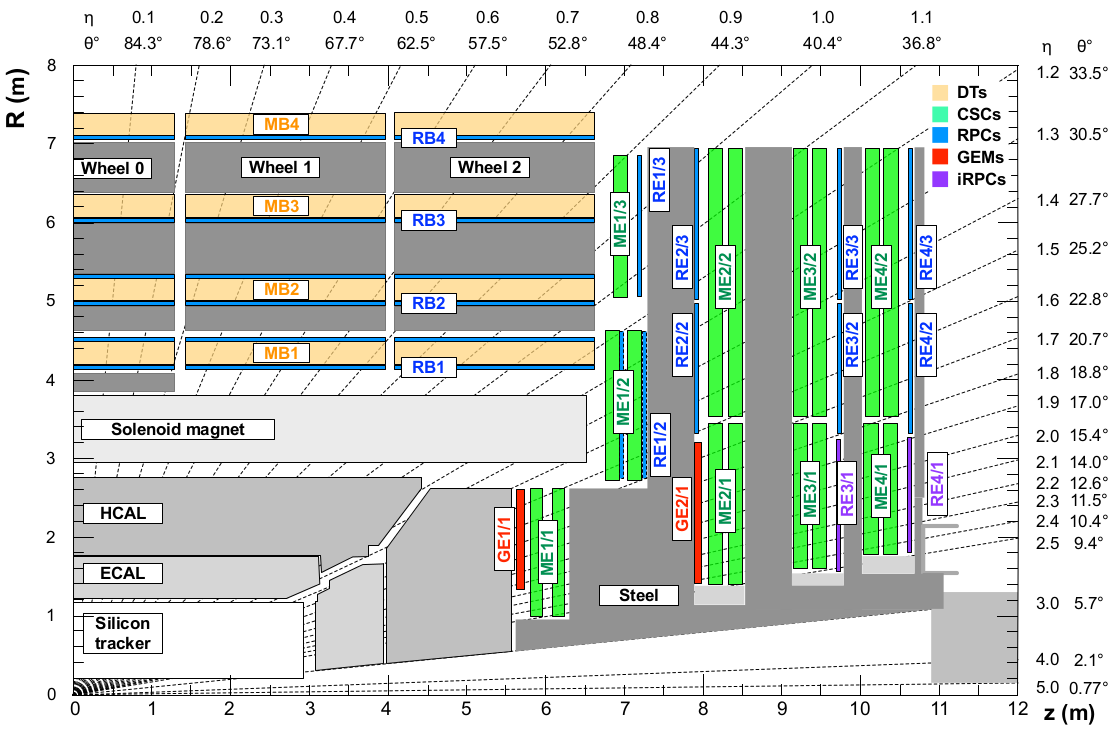
\includegraphics[width=1.0\textwidth,keepaspectratio]{figures_and_tables/rpc/muon_eta.png}
\end{center}
\caption{$\eta$ projection of the Muon System subdetectors. In purple, is labeled the iRPCS to be installed during the CMS upgrade.}\label{muons_eta}
\end{figure}

Even thought this region is covered by the CSC detectors CSC (Cathode Strip Chambers), there are some loss of efficiency due the the system geometry. The installation of additional chambers will mitigate this problem and potentially increase the global efficiency of the muon system. The new chamber, called iRPC (\textit{improved RPC}), will be different them the present one. For a luminosity of $5 \times 10^{34} cm^{-2} s^{-1}$  the neutrons, photons, electrons and positrons background in the high $|\eta|$ region is expected to by be around 700 Hz/$cm^{2}$ (for the chambers in RE3-4/1). Applying a safety factor of 3, the new chambers should support up to 2 Hz/$cm^{2}$ of gamma radiation and still keep more than 95\% of efficiency. Studies indicate, so far, that the use of High Pressure Laminates (HPL) for the double gap chambers is the most suitable choice. In order to reduce the aging and increase the rate capability, the electrodes and the gap size should be reduced in comparison with the present system.

One of the challenges for the R\&D of the iRPC chambers is measuring the their performance in a high radiation environment, as the one for HL-LHC. For this, the CMS RPC project uses the Gamma Irradiation Facility (GIF++)~\cite{gifpp}, at CERN. The GIF++ is located at the H4 beam line in EHN1 providing high energy charged particle beams (mainly muon beam with momentum up to 100 GeV/c), combined with a 14 TBq 137-Cesium source. In the GIFF++ it is possible to achieve the HL-LHC total dose in a much reasonable amount of time. With the shutdown of LHC, the muon beam source is also off and will stay like this for 3 years. This means that the only muon sources for studies in GIF++ are cosmic muons. 

In order to create a trigger system for iRPC R\&D, the usual procedure is to use scintillators, on the top and on the bottom of the chamber. This is effective, but in a high gamma radiation environment, scintillators can be very sensitive which could lead to an undesirable amount of fake triggers which can degrade the measurements. Also, if one wants to covers a large area with scintillators, this can be expensive and they will not provide any means of tracking to measuring not only the global, but also the local chamber performance.

To provide a solution, the CMS RPC got in agreement with the LHCb~\cite{lhcb} Muon Project to use their Multiwire Proportional Chambers (MWPC)~\cite{mwpc}, which were removed from LHCb, to be replaced by new chambers, and use them as trigger and/or tracking system at GIF++. This chambers, by design, have relatively low gamma sensitivity, already have some 1-dimensional resolution ($O$(cm)) and, the biggest advantage, with respect to any other gaseous particle detector option: LHCb has hundreds of vacant chambers. Any other detector would have to be build.

Not going in details of the MWPC technology nor the LHCb chamber construction~\cite{lhcb_mwpc}, these chambers have a total active area of 968 $\times$ 200 $mm^2$ divided 2 layers (top and bottom) of 24 wire pads (40 $\times$ 200 $mm^2$) composed of around 25 wires/channel, grouped by construction. Each chamber is equipped with 3 FEBs (Front-End Boards) with 16 pads each.

A channel is a logical combination of a top layer (pads) and a bottom layer readout. These readouts can be combined in AND or OR logics. One can have 8 channels per FEB, each channel being a logical combination of top and bottom pads. In this mode they are called AND2 and OR2. It is also possible to have the FEB configured in a 2 channels mode, each one corresponding to one sixth of the total readout pads. In this mode, all the pads can be combined in OR (called OR8) or they can be AND'ed in top and bottom pads and then group in OR (called OR4AND2). Figures~\ref{8channels} and~\ref{2channels} presents a logical diagram for each readout mode.

\begin{figure}[!htbp]
\begin{center}
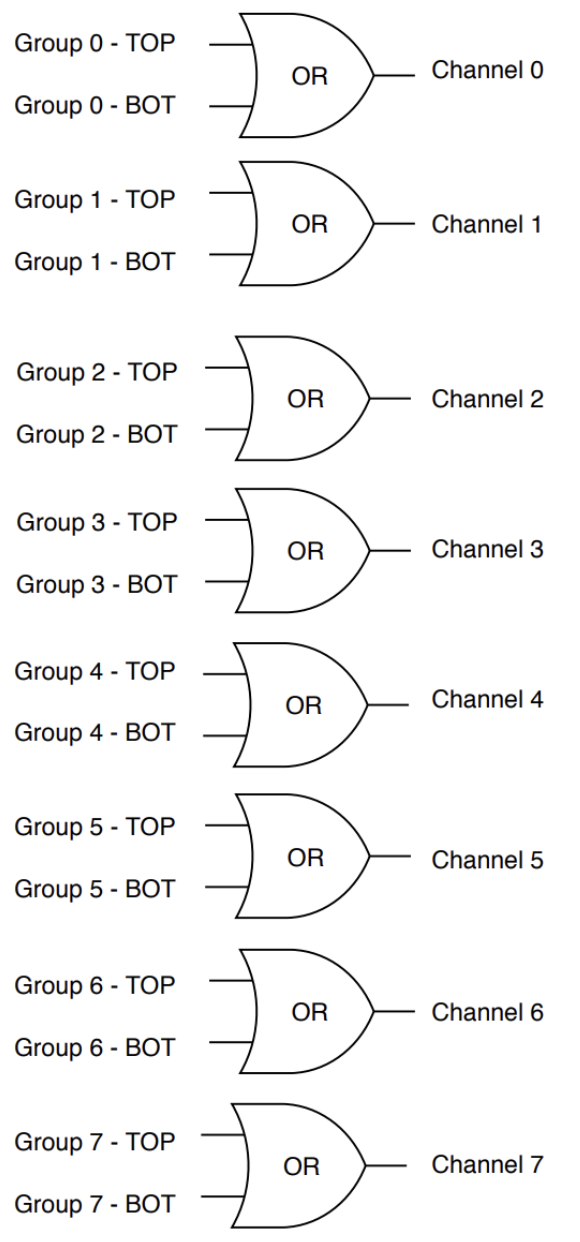
\includegraphics[width=0.27\textwidth,keepaspectratio]{figures_and_tables/rpc/mwpc/or2.png}\hspace*{1.cm}
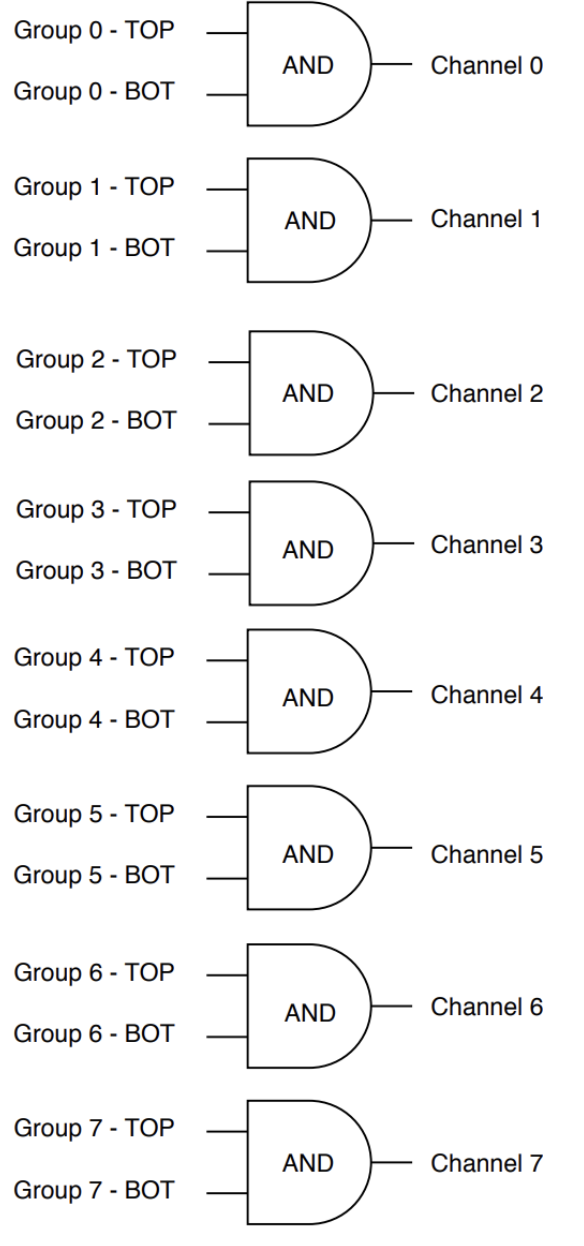
\includegraphics[width=0.27\textwidth,keepaspectratio]{figures_and_tables/rpc/mwpc/and2.png}\hspace*{1.cm}
\end{center}\vspace*{-.5cm}
\caption{FEB configured 8 channels modes. Group should be understood as wire pad. Left: Logical diagram for OR2. Right: Logical diagram for AND2.}
\label{8channels}
\end{figure}


\begin{figure}[!htbp]
\begin{center}
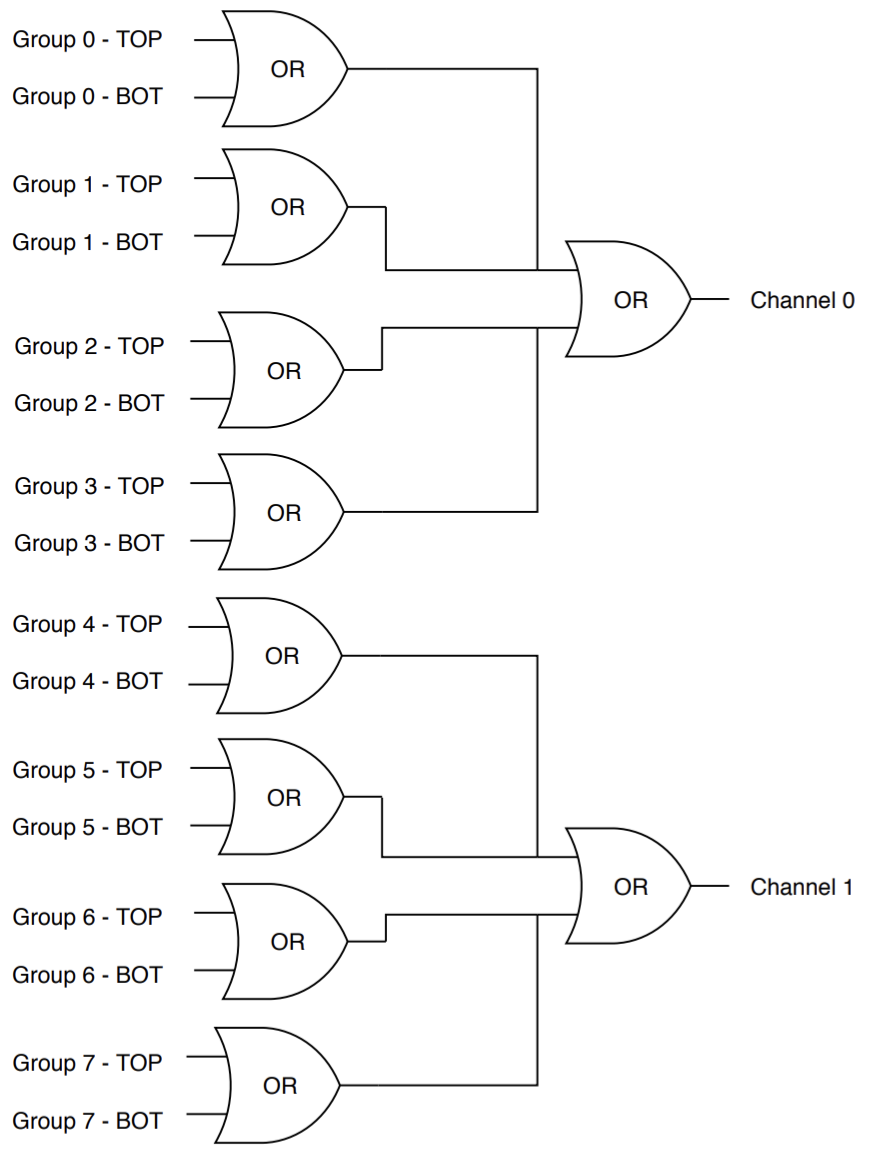
\includegraphics[width=0.40\textwidth,keepaspectratio]{figures_and_tables/rpc/mwpc/or8.png}\hspace*{1.cm}
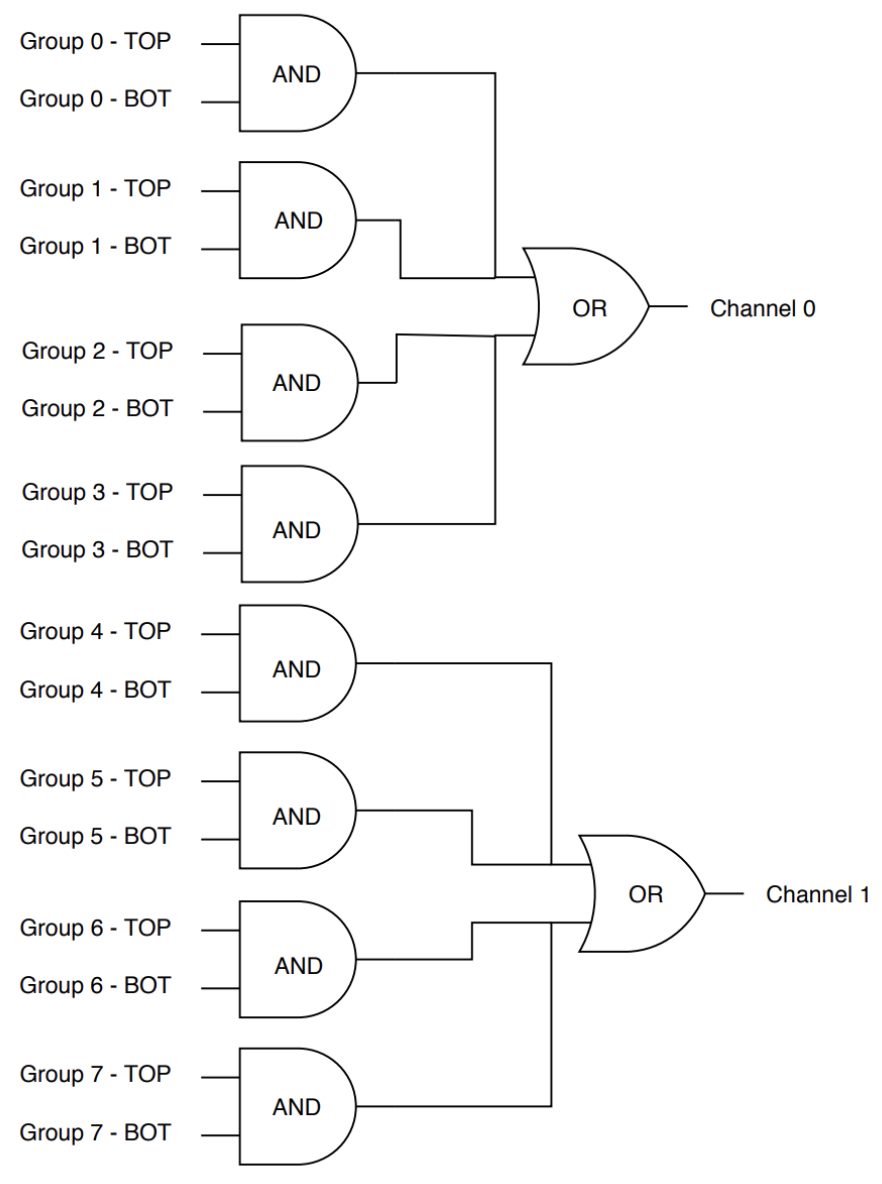
\includegraphics[width=0.40\textwidth,keepaspectratio]{figures_and_tables/rpc/mwpc/or4and2.png}\hspace*{1.cm}
\end{center}\vspace*{-.5cm}
\caption{FEB configured 2 channels modes. Left: Logical diagram for OR8. Group should be understood as wire pad. Right: Logical diagram for OR4AND2.}
\label{2channels}
\end{figure}

The nominal gas mixture for these chambers is Ar/CO2/CF4 (40:55:5). For a matter of simplicity, it was used an already available similar gas line in the same building, used by CMS CSC (Cathode Strip Chamber)~\cite{muon_tdr}, which has a similar composition (40:50:10). Optimal conditions are obtained with 2 to 4 liters/hour of gas flux and 2.65 kV of applied voltage.

Figure~\ref{setup} shows the setup that was prepared for commissioning of this chambers. It was mounted two chambers on top of another (chambers A and B) above an RPC R\&D chamber and two other chambers on the bottom (chambers C and D). These four MWPC will be used as telescope for the RPC chamber. All the services were mounted in rack, as in Figure~\ref{setup}. This includes power supply (low voltage and high voltage), distribution panel, VME crate and boards for FEB control, computer for control (high voltage, and FEB control) and NIM crate and boards for LVDS to NIM signal conversion, logics and counting.

\begin{figure}[!htbp]
\begin{center}
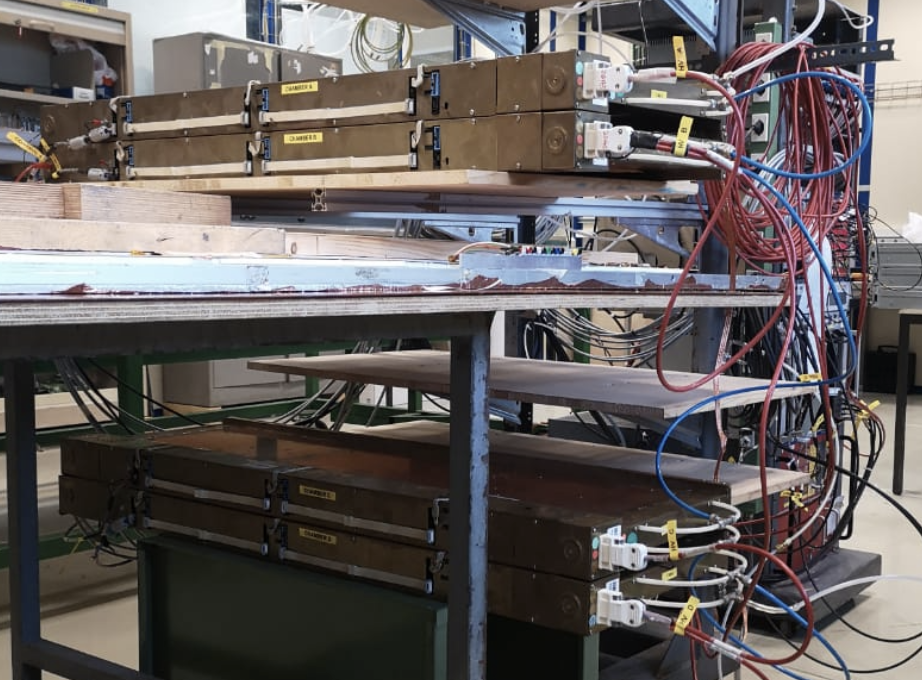
\includegraphics[width=0.57\textwidth,keepaspectratio]{figures_and_tables/rpc/mwpc/setup.png}\hspace*{1.cm}
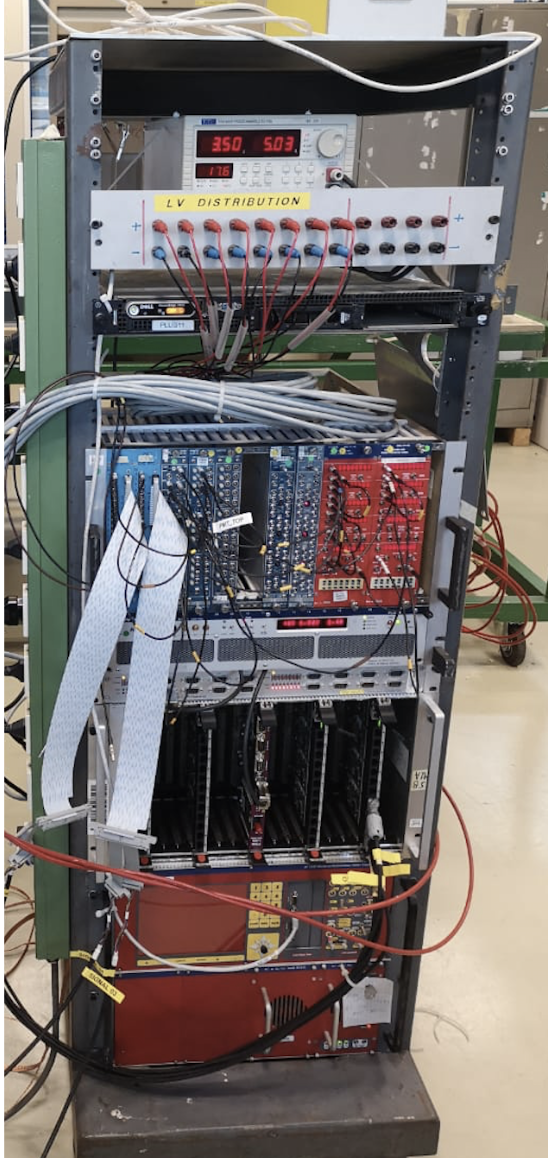
\includegraphics[width=0.23\textwidth,keepaspectratio]{figures_and_tables/rpc/mwpc/rack.png}\hspace*{1.cm}
\end{center}\vspace*{-.5cm}
\caption{Left: Setup mounted for commissioning. Two MWPC chamber on the top (chambers A and B) and two (chambers C and D) on the bottom with a RPC R\&D in the middle. Right: Rack with all the services for the operation of these chambers.}
\label{setup}
\end{figure}

Due to the short amount of time available for the commissioning, only two measurements measurements were made with these chambers. They were meant to be a proof of concept for future activities.

The first measurement was to measure the coincidence rate of two chambers as a function of the distance between the two top planes (Figure~\ref{coincidence}). This measurements were done with nominal working point, with one FEB configured in  2 channels mode with 7 pC threshold, in (160 mm x 160 mm) area per chamber. One can observe that, if we go for a telescope trigger in the order of 1 meter of separation between the chamber, the logical combination chosen has negligible effect in the coincidence rate. Also, the fits can be used to estimate the rate in a configuration with chamber on the roof and under the floor. This could be the case of a universal trigger, to be mounted in GIF++ with these chamber.

\begin{figure}[h]
\begin{center}
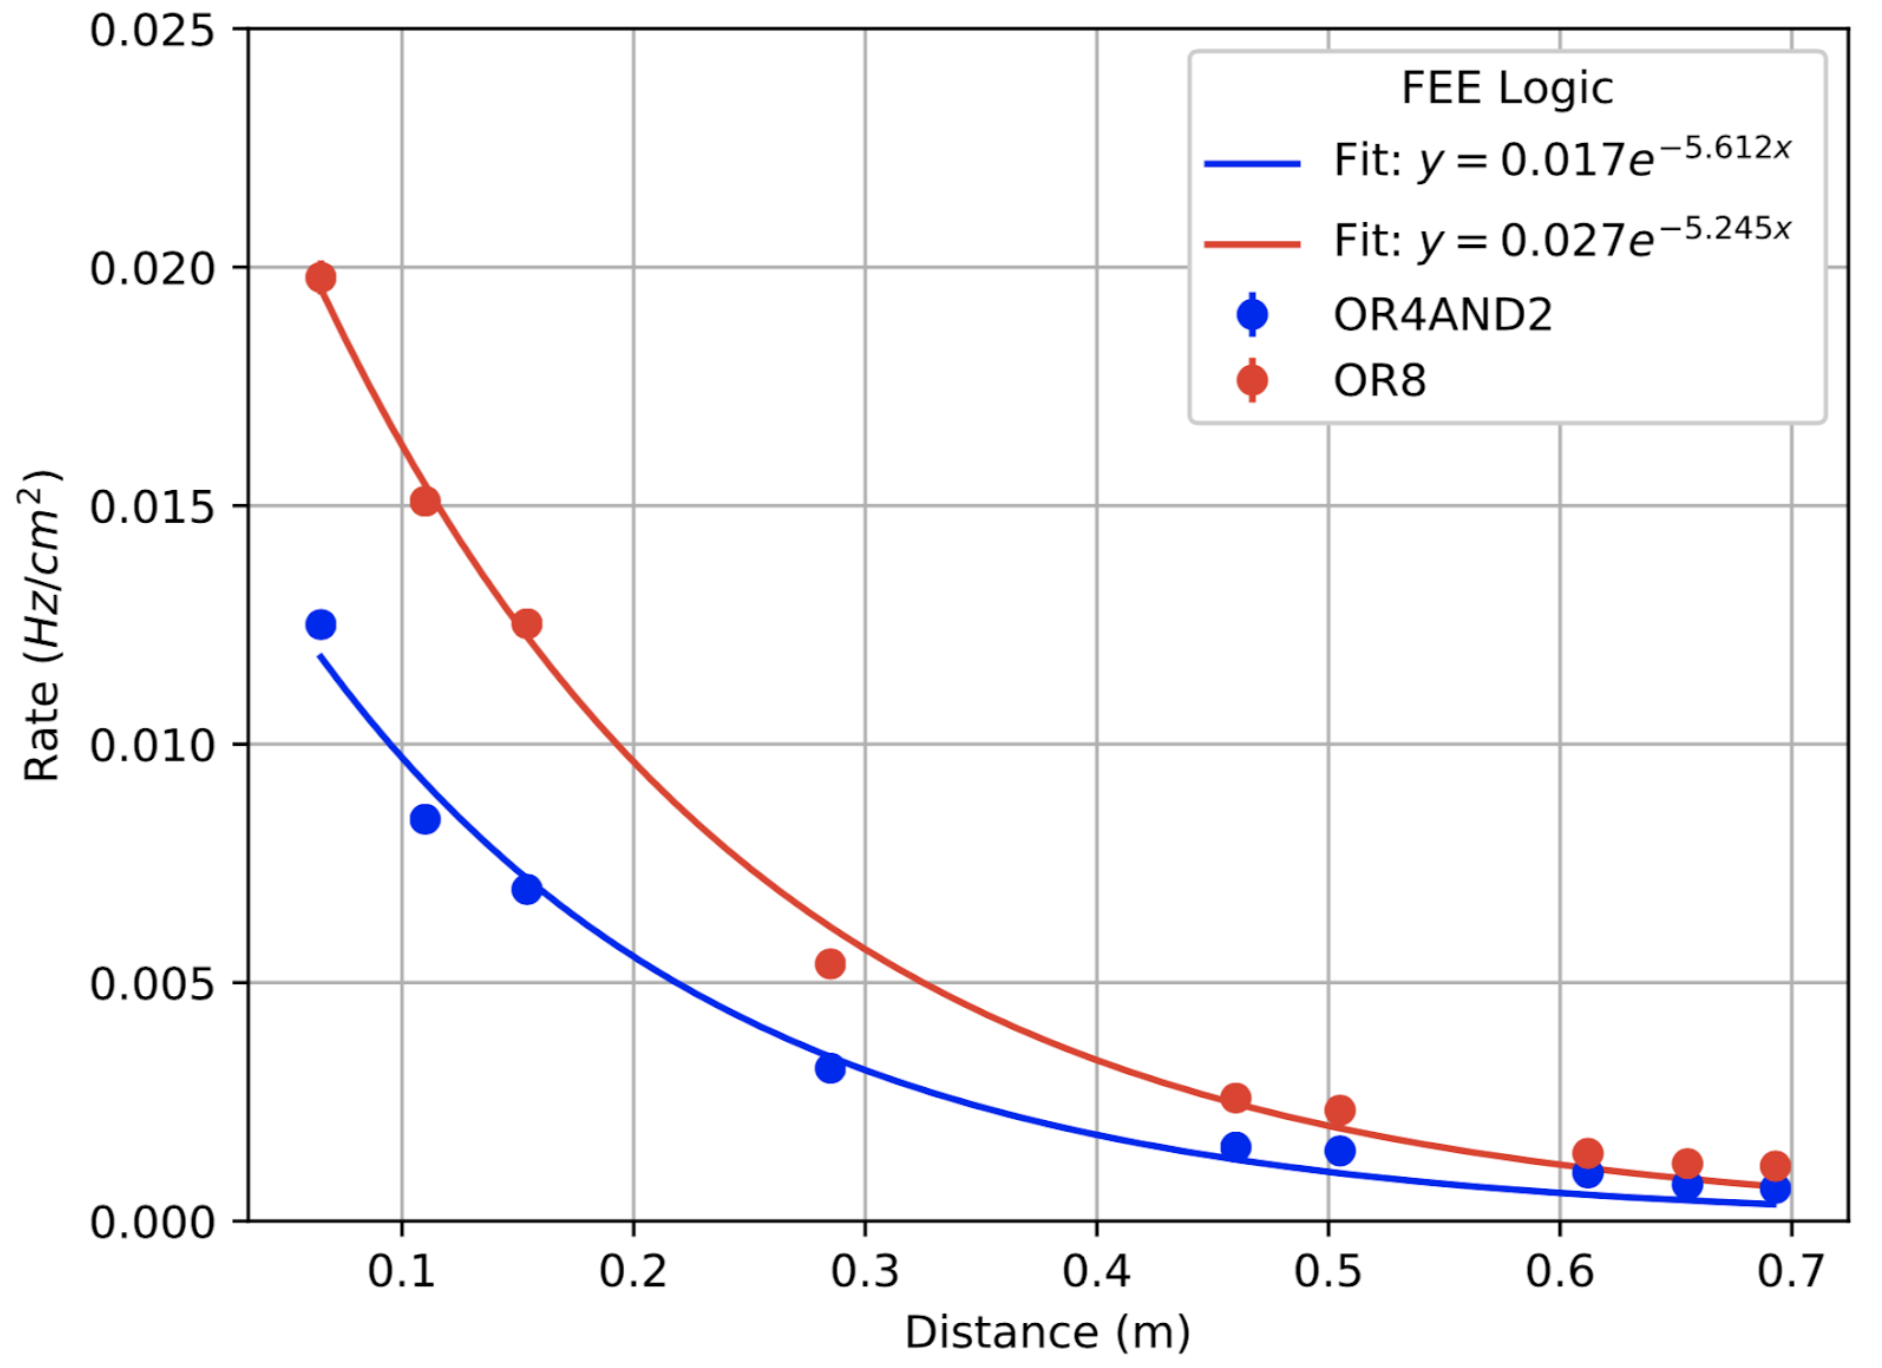
\includegraphics[width=0.7\textwidth,keepaspectratio]{figures_and_tables/rpc/mwpc/coincidence.png}
\end{center}
\caption{Coincidence rate of two chambers with respect to an arbitrary distance between the two top planes. Measured in 10 minutes, for 2 logical combinations (OR8 and OR4AND2). Applied high voltage: 2.65 kV. Threshold: 7 pC. Active area: readout of 160 mm x 160 mm per chamber.}
\label{coincidence}
\end{figure}

The second measurement consist on evaluate the impact of $\gamma$ background by placing a small Cs-137 source on top of the chamber A (Figure~\ref{gamma}). For this measurement, the distance between top planes of each pair of chamber (A to B and C to D) is 65 mm, while the distance between the top planes of A and C is 570 mm. It is clear the the $\gamma$ source has an impact on chamber A rate, but this is negligible when we take into account the coincidence between two chambers.

\begin{figure}[h]
\begin{center}
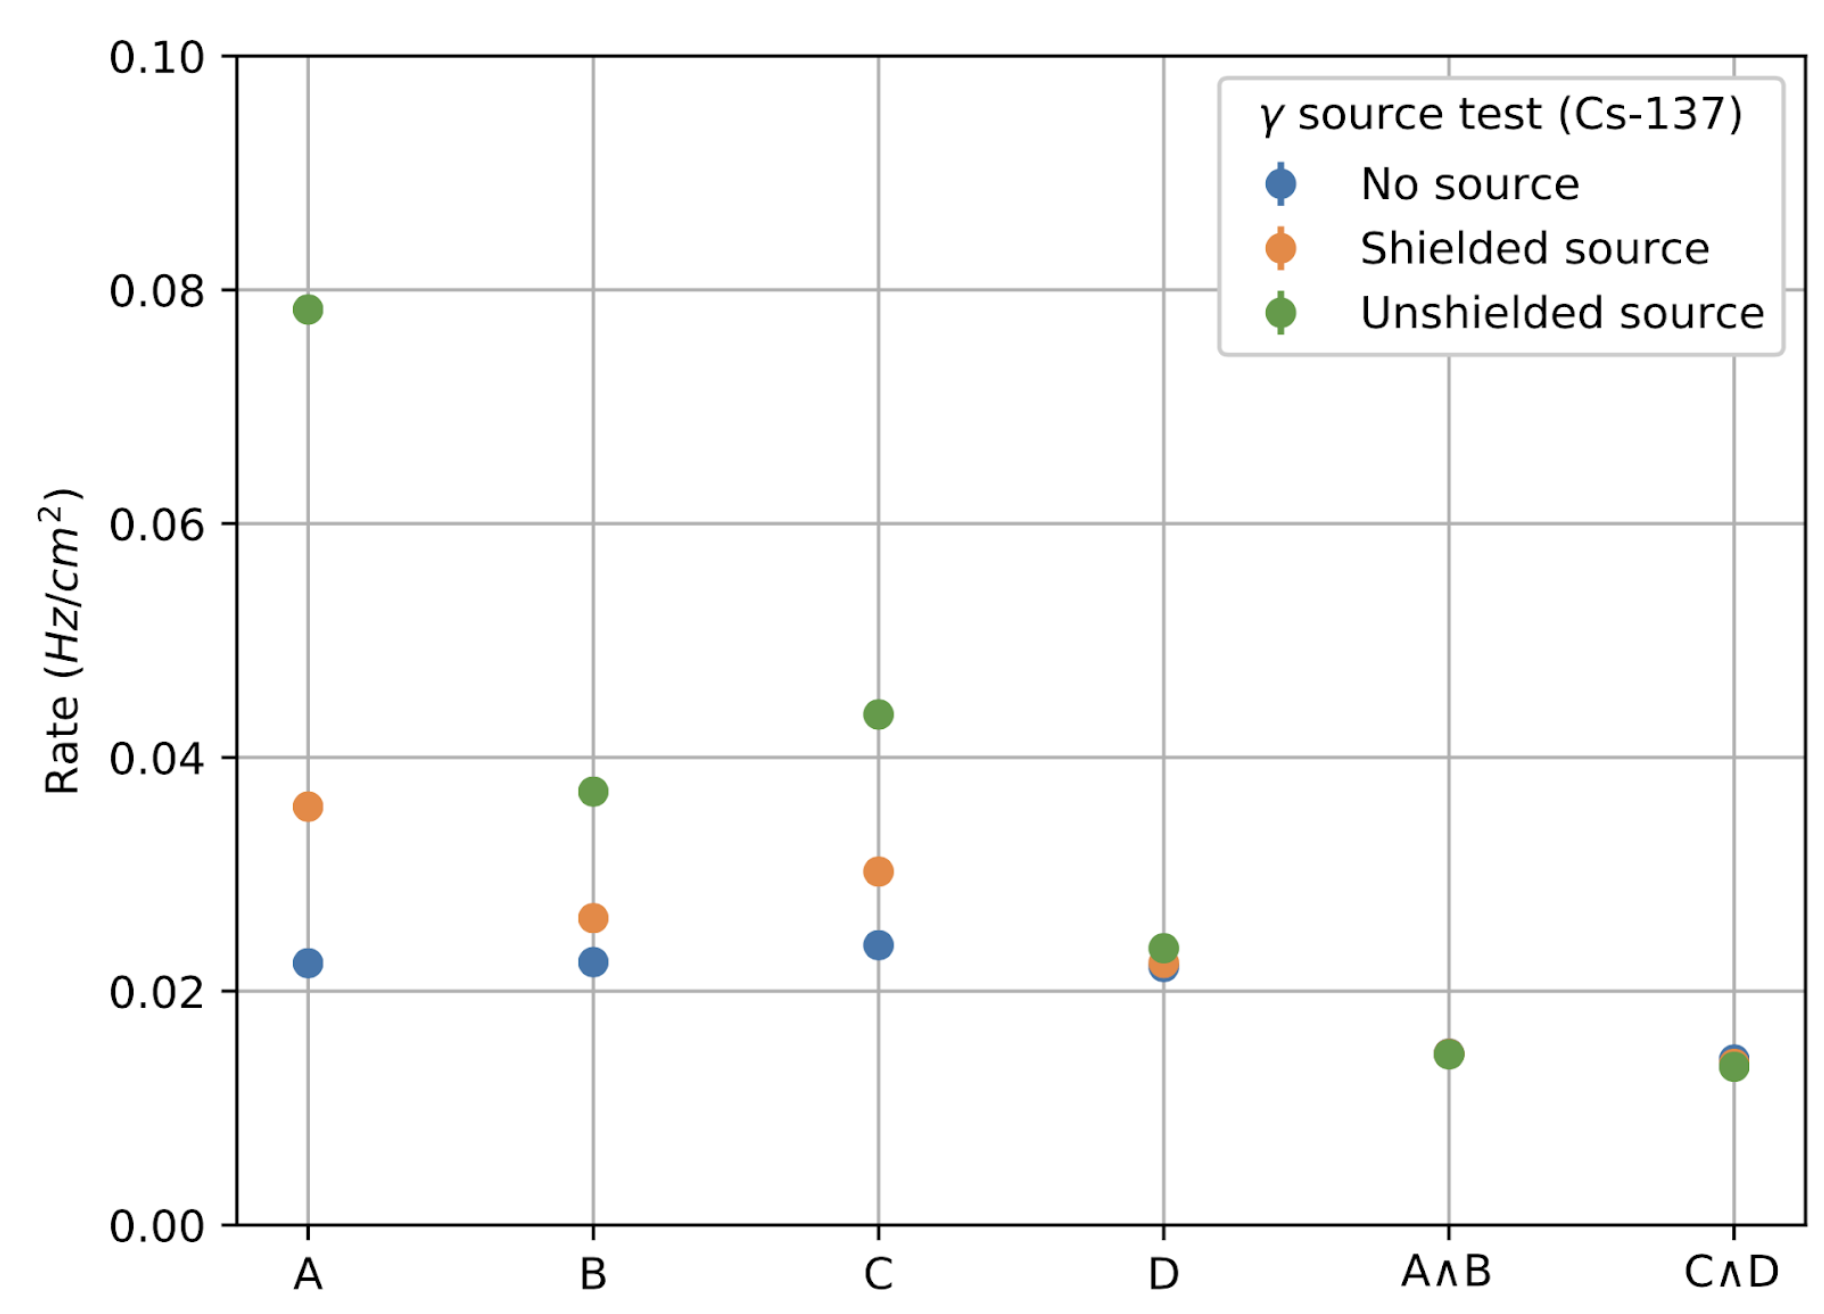
\includegraphics[width=0.7\textwidth,keepaspectratio]{figures_and_tables/rpc/mwpc/gamma.png}
\end{center}
\caption{Individual rates (chambers A, B, C and D) and coincidence rates for two chambers (A AND B, C AND D), for without $\gamma$ source (blue), a shielded $\gamma$ source (orange) and an unshielded $\gamma$ source (green). Source sitting on top of chamber A. Applied high voltage: 2.65 kV. Threshold: 7 pC. Active area: readout of 160 mm x 320 mm per chamber. Logical combination: AND2}
\label{gamma}
\end{figure}

This two measurements were enough to validate this chambers as possible trigger pro RPC R\&D with cosmic muons in the laboratory and at GIF++. The next steps would be use this MWPC chamber to implement a tracking system from triggering. This would demand some developments, since, due to bandwidth restrictions, the signal from each FEB would have to go to a programmable fast electronics, i.e. a FPGA, which would reconstruct muon tracks and provide the trigger to the DAQ system. This can be done by placing the two pair of chambers (AB and CD) in orthogonal configuration and read the signal in a CAEN V2495 board~\cite{caen_fpga}. 


\clearpage

\subsection{LS2 and the RPC Standard Maintenance}

In December 2018, the LS2 (Long Shutdown 2) was started. This a period in which the LHC and its detectors (CMS included) stop their operation for maintenance and upgrade. The LS2 will go up to 2021, when LHC and CMS restart the data taking with the Run3. 

During the LS2 it is being installed services for the new chambers (gas pipes, low voltage (LV), cables, signal and control optical fibers, high voltage (HV) cable and support equipment, and HV/LV power supplies), as well as continuity to the to the RPC R\&D studies, besides the reparation of broken elements of the present system, i.e. chamber in the barrel region which present gas leak problems, maintenance of the LV and HV connectivity and power system, maintenance of the control system of problematic chambers (Front-Ends boards, cabling and Distribution Boards) and the dismount and reinstallation of four stations in the endcap (RE4) on both sides of CMS~\cite{re4_dismount}.

What concerns the standard maintenance of the present RPC system, the main LS2 activities in which the student was involved, can be divided in three main tasks: (a) HV maintenance, (b) LV and control maintenance and (c) detector commissioning. 

\subsubsection{HV maintenance}

A key factor of and RPC performance is the applied high voltage (HV). The CMS RPC achieve their optimal performance with, around, 9.5 kV applied in each gap. This voltage is in the range of the dielectric breakdown of many gases, which could lead to potential current leakages, if some part of the system is damaged, poorly operated or badly installed. If the currents are high enough this can make impossible the operation of the chamber. In cases like this, during the operation period (data taking), the problematic HV channel is identified and turned off (each chamber has two channels, one for each lawyer of gaps). Chambers in this situation are said to be operating in single gap mode (SG).

The goal for the HV maintenance is to, now that the CMS is off and the chambers are accessible, identify which part of the HV supply system is causing the current leak and fix it the best way possible. Usually the problem is beyond the power supply, very often connectors or the gap itself are damaged.

The CMS RPCs uses two kind of HV connectors, monopolar and tripolar connector. The monopolar are used to connect the chamber to the power supply. If mounted properly, rarely they present problems. The connection to the chamber is made by tripolar connectors, in which the ground and the HV for both gaps arrives to the chamber in a single connector, for simplicity and to save space in the patch panel. Unfortunately these connectors are relatively fragile, and they could be a potential source of leak, specially if they were poorly mounted, badly operated or with aging itself. Also, since this was a connector made exclusively for the CMS RPC system, some design choices had to be improved after the installation of other chamber. Those installed with old batches of tripolar connectors are sensitive ones. The reparation of this connectors consists in isolate the connector from the chamber and power it up to 15 kV (maximum voltage allowed by the system). If the tested connector is broken one will observe a very fast increase in the current of the HV channel. The only solution to this kind of problem is to replace the connector.

On the other hand, if the connector is powered isolated and pass the test, the problem beyond the connector (assuming that the power system have already been tested), i.e. inside the chamber. When a chamber is in SG mode it means that a full layer is off, but not necessarily all the gaps in that layer are bad (a RPC can have up to three per layer). In this situation, the procedure consists in cutting the cables that comes from the gaps to the chamber side connector one by one and identify which gap of the problematic layer is the broken by powering it. Once identified, this gap should isolated and the other ones reconnected. The broken gap is unrecoverable, since it is inside the chamber, but 5\% to 10 \% of efficiency can be retaken, without changing the applied HV and increasing the longevity of the chamber.

Another contribution to the HV maintenance was the proposal of a procedure to replace the problematic tripolar connector by a monopolar (also called jupiter) connector, which are known for being much more stable and reliable. The figure~\ref{jupiterized} (left) show the designed adapter for the chamber patch panel which would made this change possible. Figure~\ref{jupiterized} (right) shows a tryout of a chamber in which this procedure was tested. The proposal was presented to the RPC community and approved to be used from now on. Technical drawings and instructions were provided.

\begin{figure}[!htbp]
\begin{center}
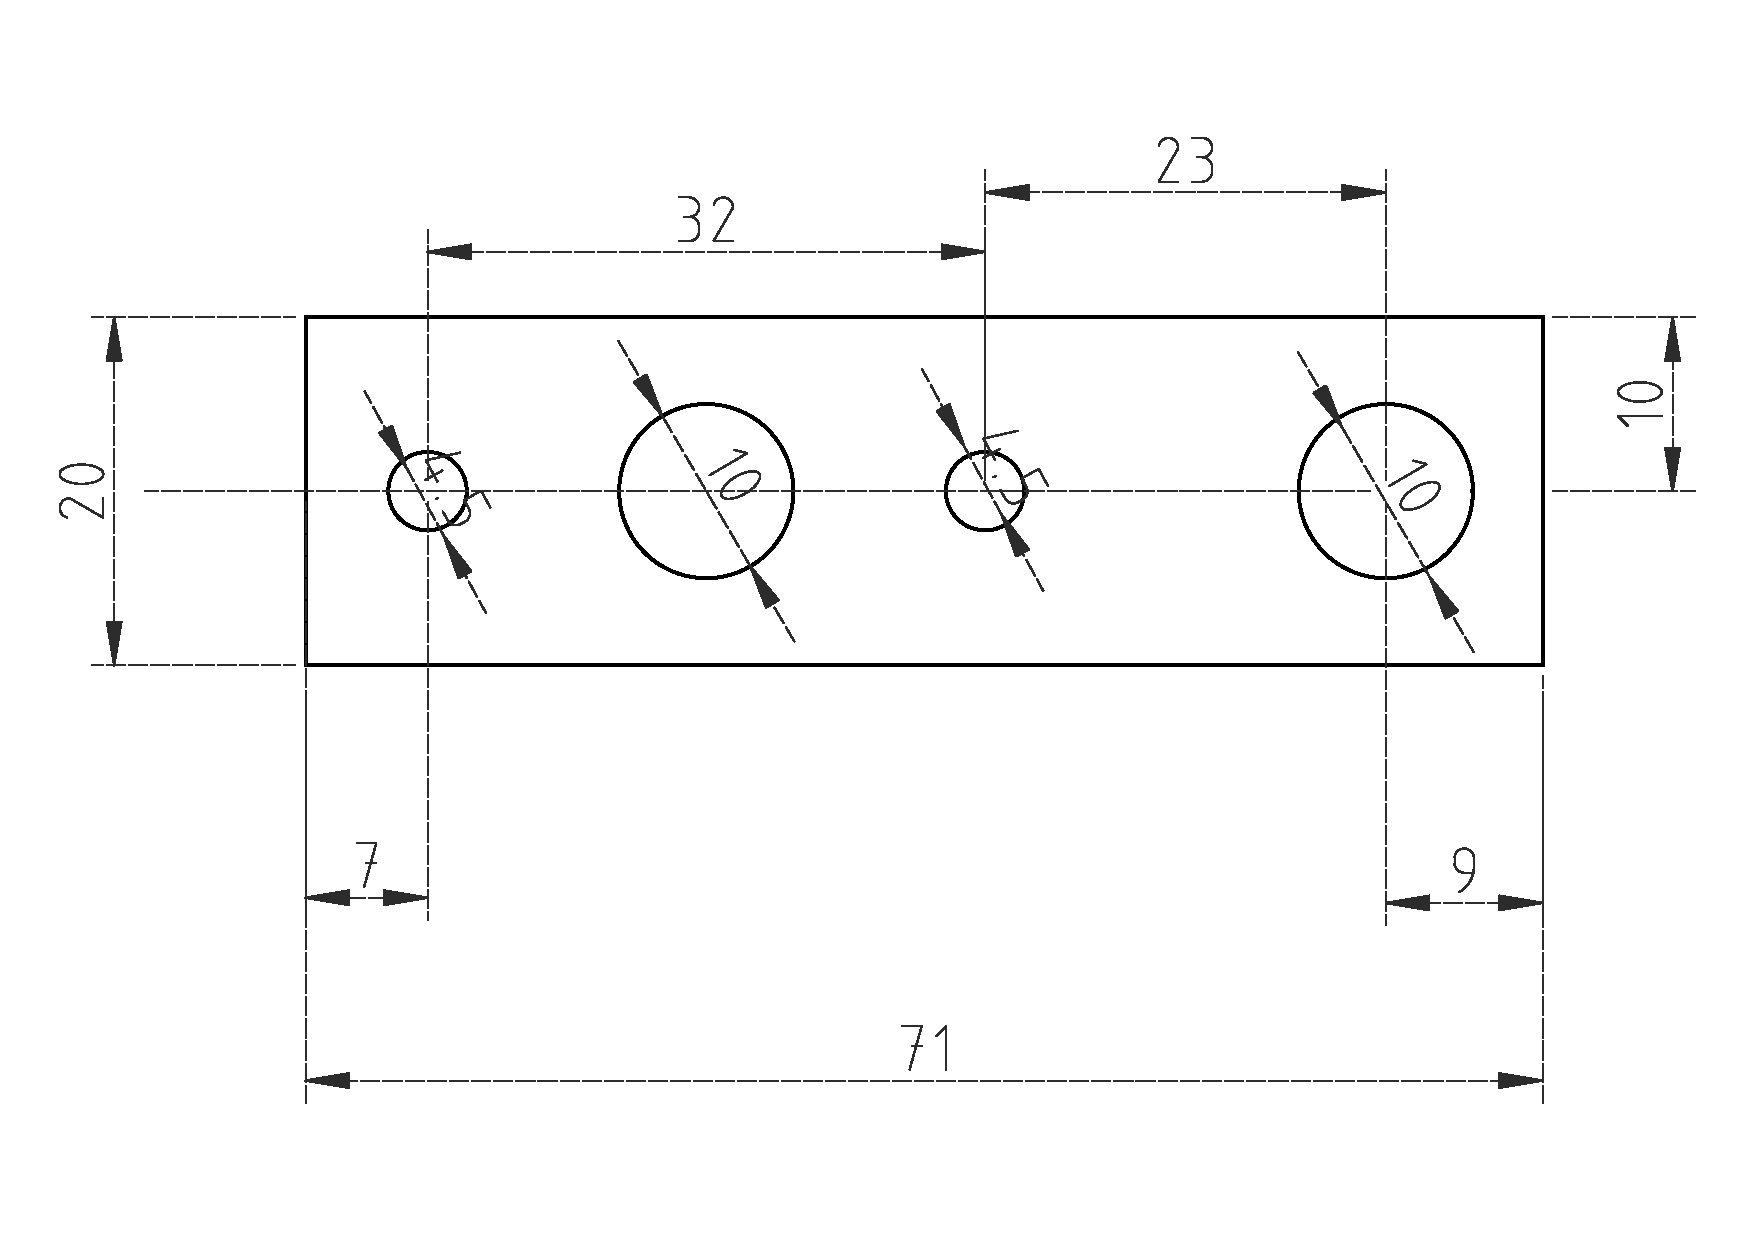
\includegraphics[width=0.45\textwidth,keepaspectratio]{figures_and_tables/rpc/endcap_hv_pp.pdf}\hspace*{1.cm}
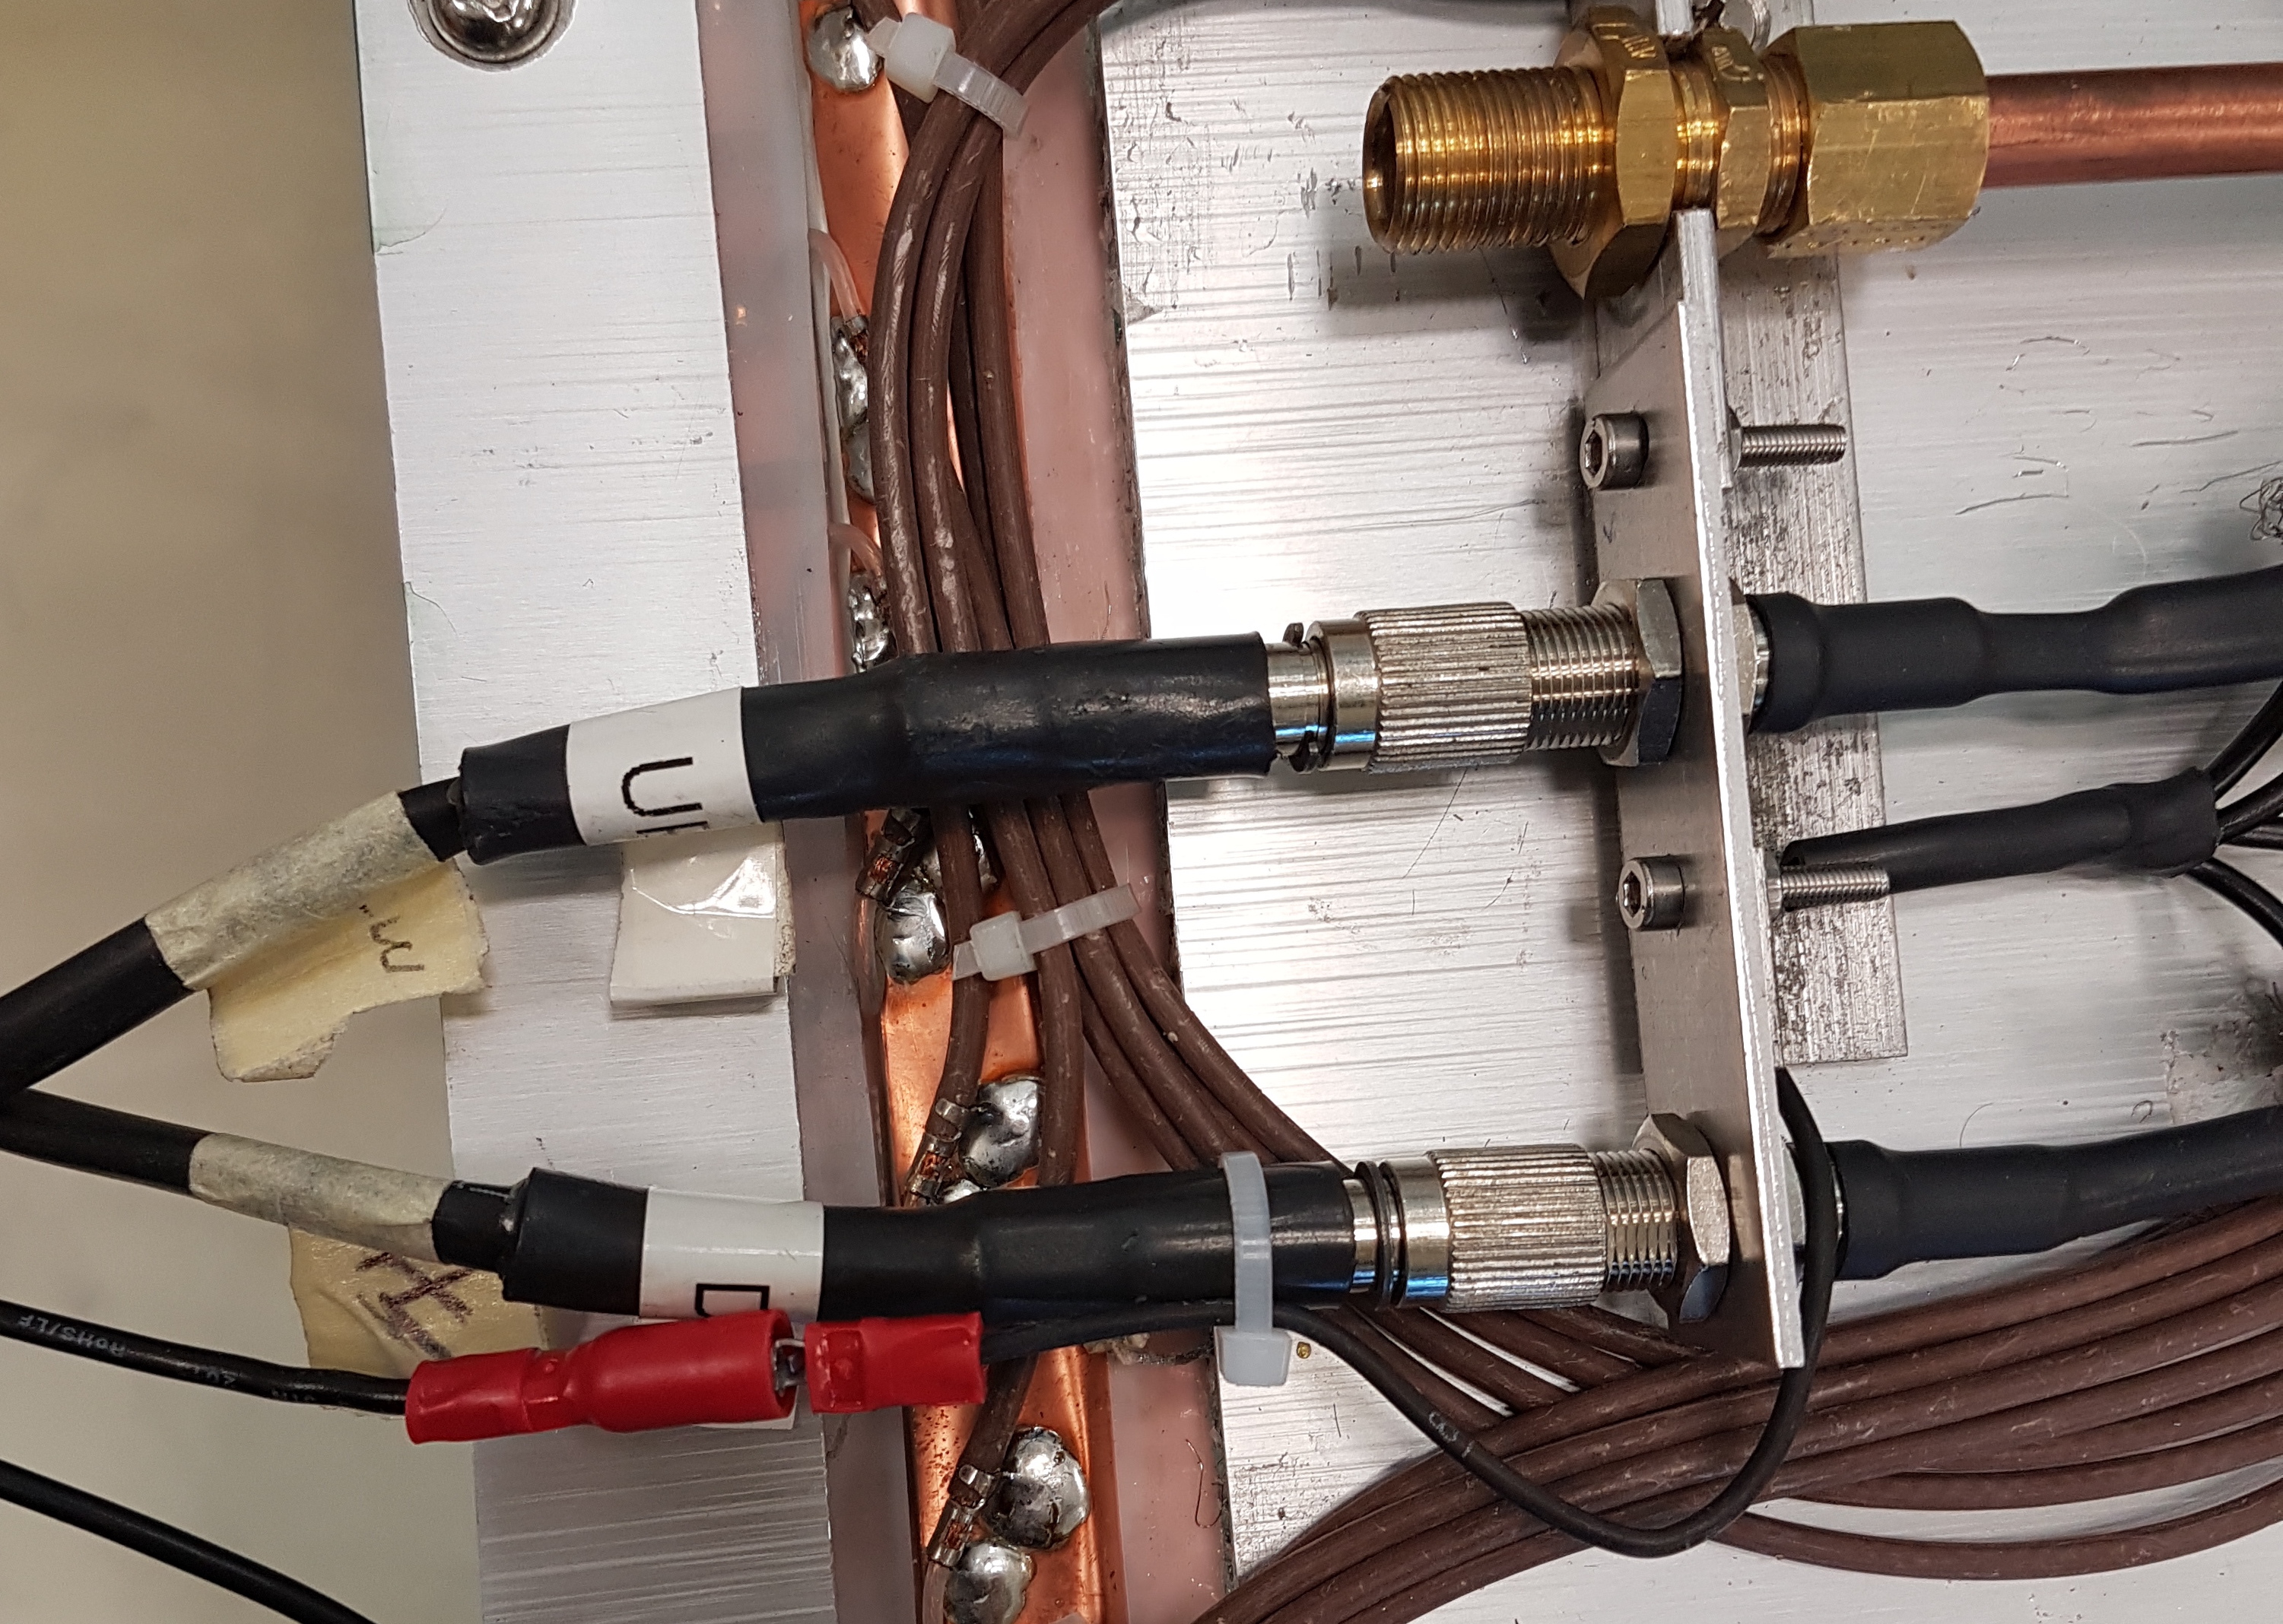
\includegraphics[width=0.45\textwidth,keepaspectratio]{figures_and_tables/rpc/endcap_hv_pp_tryout.jpg}\hspace*{1.cm}
\end{center}\vspace*{-.5cm}
\caption{Left: Proposed adapter the chamber patch panel which make it possible to replace a tripolar by a jupiter HV connector. Right: Try out of the proposed HV connector replacement.}
\label{jupiterized}
\end{figure}

\subsubsection{LV and control maintenance}

The low voltage (LV) and control maintenance consists in make sure that the Front-End Boards (FEBs) are powered and configurable, which means that the LV power system is working from supply board to the cable, that the signal cables are in good state and properly connected to the chamber and to the link boards and that the on-detector electronics (FEBs and Distribution Boards - DBs) are working fine.

Usually, this system is very reliable. The weak point, in most of the cases, is the detector electronics. When a FEB~\cite{rpc_feb} (as in Figure~\ref{rpc_feb}) is problematic it can present regions of very high noise or no signal at all (silent), which can not be recovered by the threshold control. In cases like this, when the FEB is accessible, it can be replaced in order to recover efficiency in the problematic chamber. This procedure is done by extracting the chamber from inside the detector (only for barrel chamber) and opening its cover to have access to the problematic component. Removed boards are send back to production labs for refurbishment.

\begin{figure}[h]
\begin{center}
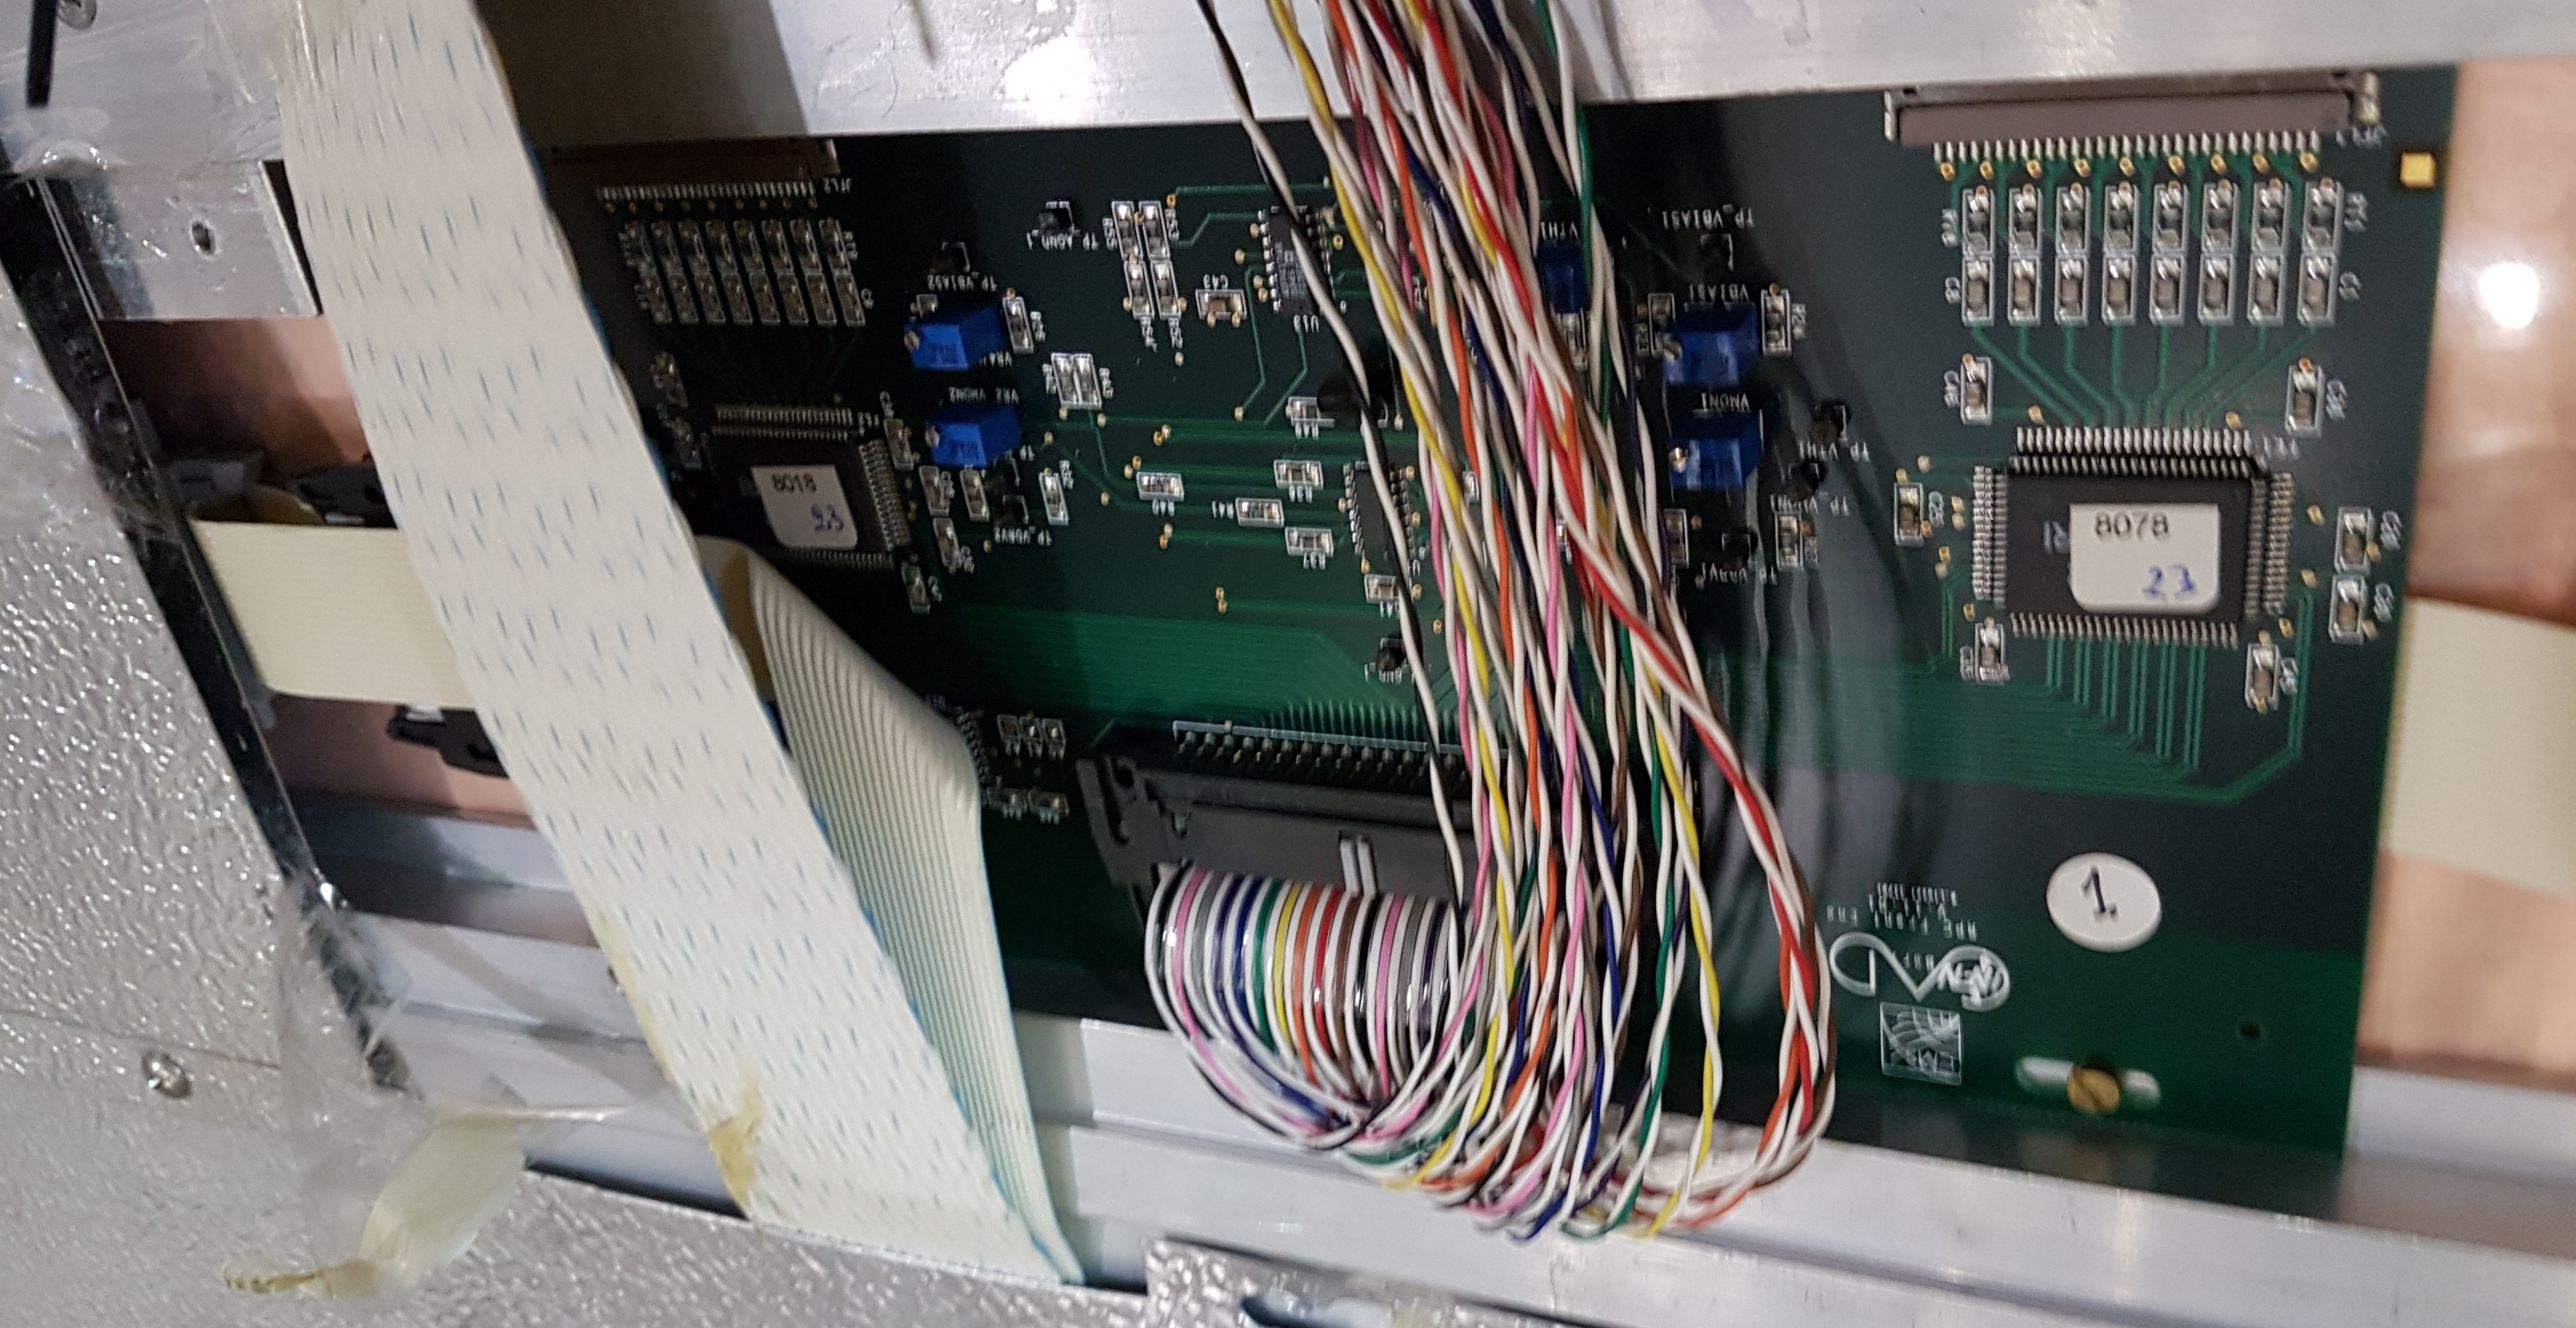
\includegraphics[width=0.7\textwidth,keepaspectratio]{figures_and_tables/rpc/rpc_feb.jpg}
\end{center}
\caption{RPC Front-end board (FEB) used in the barrel chambers.}\label{rpc_feb}
\end{figure}

The most usual problem is a chamber in which the threshold control was lost. For those chamber, most probably, the problem is in the distribution board of the chamber, which is a piece of hardware responsible for distribute the LV power to the FEBs (3 to 6 per chamber) and send the threshold control signal to the FEBs via I2C line. If a chamber has no threshold control, it means that the RPC operation has no control over the signal selection, which can potentially induce performance issues. 

For the barrel this maintenance happens concomitantly with the gas leak reparations on the barrel chamber, since both demands the chamber extraction, which is a complex procedure in terms of operation and demands specialized equipment and manpower. For technical reasons, the gas leak extractions have precedence over LV ones.



\subsubsection{Detector commissioning}
 
All the LS2 activities demands uncabling of the chamber to be repaired and possibly some neighbor chambers. Also, it can involve the replacement of components of the chamber. To avoid damage to the system a compromising procedure is needed after all this activities. Given the responsibilities of the commissioning it was necessary to: (a) make sure that the the RPC system keep tracks of all the interventions, (b) maintain all the algorithms used in the commissioning procedure, (c) together with the RPC Coordination, define a pool of people and a schedule to the commissioning of the system and (d) follow-up, with other CMS RPC experts, the availability of materials and resources for the commissioning operations.

Besides the organizational tasks, the commissioning demanded to establish procedures to ensure the connectivity and functionality of HV and LV connections. For the HV, it is needed to make sure that the chambers are properly connected, without miscabling~\footnote{Mixed cable connections.} and that the currents at stand-by HV  and working point HV are compatible with the ones in the end of last data-taking (end of 2018). This activity will start in November/2019, when the CMS RPC Standard Gas Mixture will be available again.
 
For the LV point of view, the LV power cable and signal cables should also be properly connected, and presenting a noise profile compatible with last data-taking. One key point for this task is to make sure that that there are no miscabling of signal cable. One RPC chamber can have from 6 to 18 signal cable, which are connected very close one to another. There is a good chance that a chamber, after reparation, have its signal cables mixed. In order to diagnose situations like this, it was validated a algorithm present in the RPC Online Software, but never used since LS1, which, by changing the threshold of each component of the RPC system, from very high to very low values (component by component), can spot miscabled chambers. Since the control line is independent of the signal line, a misclabed will present a different noise from what is expected.

Besides the validation of this algorithm, it was also implemented a web system (Figure~\ref{comm}), developed in Flask~\cite{flask} wich automatize the execution of the algorithm, making transparent to the shifter (or the one performing the commissioning) the procedure to get miscabling report.

\begin{figure}[h]
\begin{center}
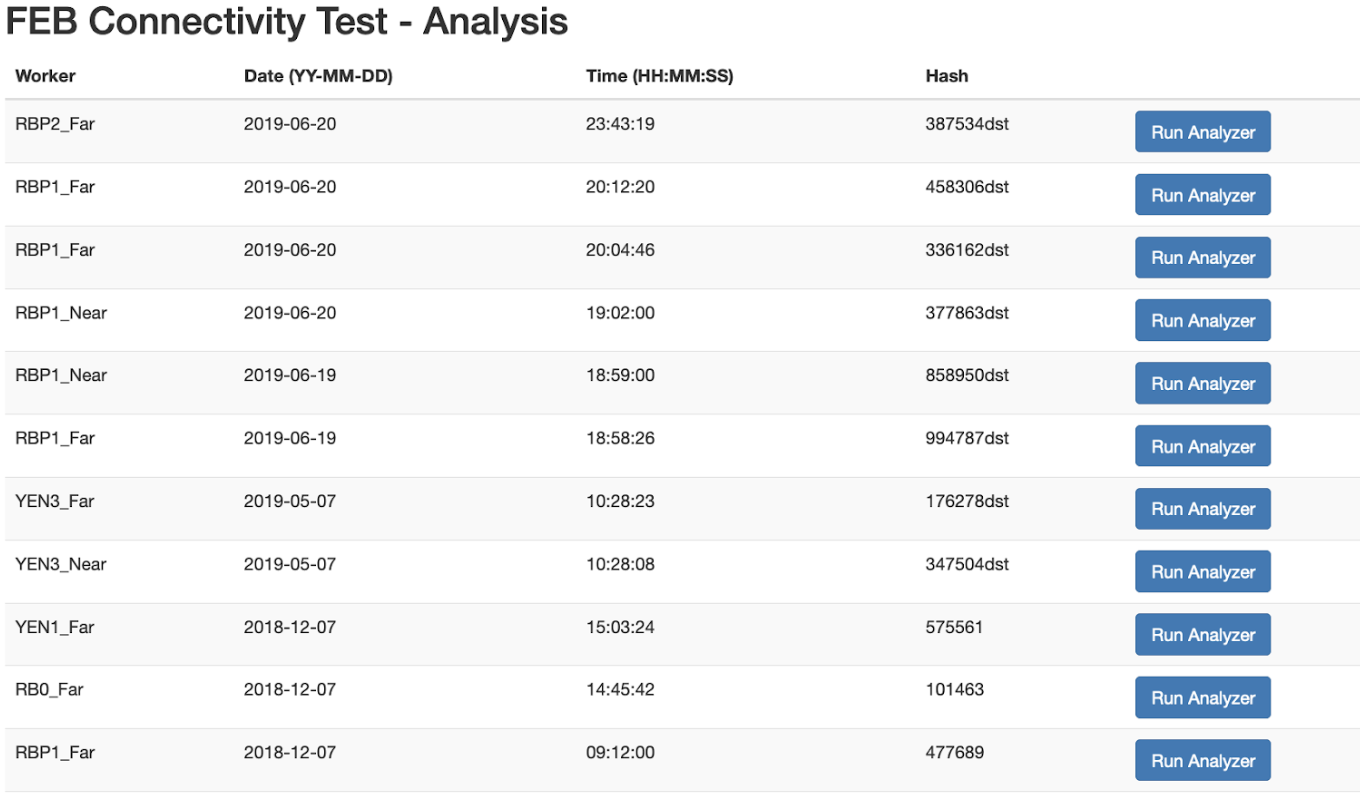
\includegraphics[width=0.7\textwidth,keepaspectratio]{figures_and_tables/rpc/comm.png}
\end{center}
\caption{RPC FEB Commissioning Analyzer.}\label{comm}
\end{figure}

The LV commissioning is ongoing, since it happens, as much as possible, right after the chamber reparation.

\clearpage